%%=====================================================================================
%%
%%          ToDo :  !!! important !!! on debian based systems you have to install
%%                  biber with sudo apt-get install biber for the bibliography or use 
%%                  bibtex instead but biber/biblatex has utf8 support per default
%%       Filename:  main.tex
%%
%%    Description:  ESK Lab Thesis Template  
%%
%%        Version:  1.0
%%        Created:  25.08.2015
%%       Revision:  none
%%
%%         Author:  B.Eng. Oliver Kehret, okehret@stud.hs-offenburg.de
%%   Organization:  HS Offenburg, Offenburg, Germany
%%      Copyright:  Copyright (c) 2015, B.Eng. Oliver Kehret
%%
%%          Notes:  Inspired by Andreas Walz, Tobias Neff and Karl Voith
%%                
%%=====================================================================================
%---------------------------------------------------------------------------------------------------
% Settings
%---------------------------------------------------------------------------------------------------
\newcommand{\mypapersize}{A4}
\newcommand{\mylaterality}{oneside}
%% "oneside" or "twoside"
\newcommand{\mydraft}{false}
%% "true" or "false"
\newcommand{\myparskip}{half}
%% e.g., "no", "full", "half", ...
\newcommand{\myBCOR}{10mm}
\newcommand{\myfontsize}{11pt}   
\newcommand{\mylinespread}{onehalfspacing} 
%% e.g.onehalfspacing, doublespacing, singlespacing
%% Line spacing in %/100. For example 1.5 means 150% of the usual line
%% spacing. Please use with caution: 100% ("1.0") is fine because the
%% font was designed for it.
\newcommand{\mylanguage}{ngerman,american}
%% NOTE: The *last* language is the active one!
%% BibLaTeX-settings: (see biblatex reference for further description)
\newcommand{\mybiblatexstyle}{numeric}
%% e.g., "alphabetic", "authoryear", ...
%% The biblatex style which is being used for referencing. See
%% biblatex documentation for further details and more values.
%%
%% CAUTION: if you change the style, please check for (in)compatible
%%          "biblatex" package options in the file
%%          "template/preamble.tex"! For example: "alphabetic" does
%%          not have an option "dashed=..." and causes an error if it
%%          does not get removed from the list of options.

\newcommand{\mybiblatexdashed}{false}  %% "true" or "false"
%% If true: replace recurring reference authors with a dash.

\newcommand{\mybiblatexbackref}{true}  %% "true" or "false"
%% If true: create backward links from reference to citations.

\newcommand{\mybiblatexfile}{bib/bibliography.bib}
%% Name of the biblatex file that holds the references.

\newcommand{\mydispositioncolor}{0,0,0}
%% e.g., "30,103,182" (blue/turquois), "0,0,0" (black), ...
%% Color of the headings and so forth in RGB (red,green,blue) values.

\newcommand{\mycolorlinks}{false}  %% "true" or "false"
%% Enables or disables colored links (hyperref package).
\newcommand{\mytodonotesoptions}{disable}
%% e.g., "" (empty), "disable", ...
%% Options for the todonotes-package. If "disable", all todonotes will
%% be hidden (including todos).
%% ========================================================================
%%  Document metadata
%% ========================================================================
%% general metadata:
\newcommand{\myauthor}{Steve Wagner}  %% also used for PDF metadata
% (hyperref)
\newcommand{\myformation}{EI-3nat}
\newcommand{\mytitle}{Bachelor Thesis}  %% also used for PDF metadata (hyperref)
\newcommand{\mysubject}{Extension and Integration of an Abstract Interface to Cryptography Providers}  %% also used for PDF metadata (hyperref)
\newcommand{\mykeywords}{<++keywords++>}  %% also used for PDF metadata (hyperref)
%% this information is used only for generating the title page:
\newcommand{\myworktitle}{Bachelor thesis}  %% official type of work like ``Master theses''
\newcommand{\mygrade}{Bachelor of Engineering} %% title you are getting with this work like ``Master of ...''
\newcommand{\mystudy}{Electronik und Informationstechnik} %% your study like ``Arts''
\newcommand{\myuniversity}{Offenburg University of Applied Sciences} %% your
% university/school
\newcommand{\myinstitute}{Institute of reliable Embedded Systems and
Communication Electronics (ivESK)}
%% affiliation
\newcommand{\myinstitutehead}{Prof. Dr. Axel Sikora} %% head of institute 
\newcommand{\mysupervisor}{Dipl.-Phys. Andreas Walz} %% your supervisor
\newcommand{\myevaluator}{myprof} %% your evaluator
\newcommand{\myhomestreet}{street} %% your home street (with house number)
\newcommand{\myhometown}{town} %% your home town
\newcommand{\myhomepostalnumber}{psn} %% your postal number of home town
\newcommand{\mysubmissionmonth}{month} %% month you are handing in
\newcommand{\mysubmissionyear}{year} %% year you are handing in
\newcommand{\mysubmissiontown}{\myhometown} %% town of handing in (or \myhometown)
%% additional information for generic_documentation title page

%---------------------------------------------------------------------------------------------------
% formating
%---------------------------------------------------------------------------------------------------

\newcommand{\clearemptydoublepage}{\clearpage\newpage\thispagestyle{empty}\cleardoublepage}

\newcommand{\CRule}{\rule{0.95\textwidth}{0.5pt}} % New command to make the lines above figure captions


%---------------------------------------------------------------------------------------------------
% fixme makro
%---------------------------------------------------------------------------------------------------

%\newcommand{\fixme}[1]{\textbf{\large FIXME: #1}}
%\newcommand{\todo}[1]{\textbf{\large TODO: #1}}
%\newcommand{\idea}[1]{\textbf{IDEA: #1 ~\\}}


%---------------------------------------------------------------------------------------------------
% names
%---------------------------------------------------------------------------------------------------

\newcommand{\gci}{Generic Cryptographic Interface (GCI)\xspace}
\newcommand{\embtls}{emb::TLS\xspace}
\newcommand{\tomcrypt}{LibTomCrypt\xspace}
\newcommand{\vaultic}{VaultIC\num{460}\xspace}
\newcommand{\Table}{Table}
\newcommand{\Tables}{Tables}
\newcommand{\Figure}{Figure}
\newcommand{\Figures}{Figures}
\newcommand{\Subfigure}{Subfigure}
\newcommand{\Section}{Section}
\newcommand{\Sections}{Sections}
\newcommand{\Chapter}{Chapter}
\newcommand{\Chapters}{Chapters}
\newcommand{\Equation}{Equation}
\newcommand{\Equations}{Equations}

\newcommand{\Appendix}{Appendix}
\newcommand{\Appendices}{Appendices}
\newcommand{\Ref}{Ref.}
\newcommand{\Refs}{Refs.}

%---------------------------------------------------------------------------------------------------
% units
%---------------------------------------------------------------------------------------------------

\newcommand{\Hz}	{\ensuremath{\mathrm{Hz}}\xspace}
\newcommand{\kHz}	{\ensuremath{\mathrm{kHz}}\xspace}
\newcommand{\MHz}	{\ensuremath{\mathrm{MHz}}\xspace}

\newcommand{\cm}{\ensuremath{\mathrm{cm}}\xspace}
\newcommand{\m}{\ensuremath{\mathrm{m}}\xspace}
\newcommand{\mm}{\ensuremath{\mathrm{mm}}\xspace}
\newcommand{\microm}{\ensuremath{\mu\mathrm{m}}\xspace}
\newcommand{\s}{\ensuremath{\mathrm{s}}\xspace}
\newcommand{\musec}{\ensuremath{\mu\mathrm{s}}\xspace}


%---------------------------------------------------------------------------------------------------
% include figures
%---------------------------------------------------------------------------------------------------
\newcommand{\myfig}[5]{
%% example:
% \myfig{}%% filename in figures folder
%       {width=0.5\textwidth,height=0.5\textheight}%% maximum width/height, aspect ratio will be kept
%       {}%% caption
%       {}%% optional (short) caption for list of figures
%       {}%% label
\begin{figure}%[htp]
  \begin{center}
     \includegraphics[keepaspectratio,#2]{figures/#1}
     \caption[#4]{#3}
     \label{#5} %% NOTE: always label *after* caption!
  \end{center}
  
\end{figure}
}



%% ========================================================================
%%  preamble
%% ========================================================================
%_____________________________________________________________________________________
%
%       Filename:  preamble.tex
%
%    Description:  Thesis Template HS Offenburg
%
%        Version:  1.0
%        Created:  13.11.2015
%       Revision:  none
%
%         Author:  B.Eng. Oliver Kehret, okehret@stud.hs-offenburg.de
%   Organization:  HS Offenburg, Offenburg, Germany
%      Copyright:  Copyright (c) 2015, B.Eng. Oliver Kehret
%
%          Notes:  Inspired by Andreas Walz, Tobias Neff and Karl Voith
%                
%_____________________________________________________________________________________
\documentclass[]{beamer}
\usetheme{Madrid}

%_____________________________________________________________________________________
% General presentation
%_____________________________________________________________________________________
% full utf8 character set
\usepackage[utf8]{inputenc}
% language adaptions, change in main.tex (english, ngerman, american)
\usepackage[\mylanguage]{babel}									
% encode characters better, so that they can be copied out of .pdf in one piece
\usepackage[T1]{fontenc}    
% nicer quotes  
\usepackage[%
            autostyle,          % adapts language setting
            strict,             % turns warnings into errors 
            english=american    % use american quotes style
]{csquotes}
%_____________________________________________________________________________________
% Selection of useful packages
%_____________________________________________________________________________________
%
%_____________________________________________________________________________________
% SIUNITSX -- simplified usage of SI-units
%_____________________________________________________________________________________
\usepackage[% 
            exponent-product = \cdot % use \cdot instead * for exponent product
]{siunitx}	              
%_____________________________________________________________________________________
% ifthen and todonotes puts to-do-notes in the printed document if you want 
%_____________________________________________________________________________________
% used to disable todonotes package
\usepackage{ifthen}                                         
% pre-define ifthen-boolean variables:
\newboolean{myaddcolophon}
\newboolean{myaddlistoftodos}
%
% currently american is not supported by todonotes but english is fine as it's only
% effects todonotes and missingfigures
\usepackage[\mytodonotesoptions,english]{todonotes}
%_____________________________________________________________________________________
% Sourcecode printing
%_____________________________________________________________________________________
\usepackage{listings}				% include source code
									% ftp://ftp.tex.ac.uk/tex-archive/macros/latex/contrib/listings/listings.pdf
\lstset{% 							% options for representation of source code
  backgroundcolor=\color{light-gray},   % choose the background color; you must add \usepackage{color} or \usepackage{xcolor}
  basicstyle=\footnotesize,        % the size of the fonts that are used for the code
  breakatwhitespace=false,         % sets if automatic breaks should only happen at whitespace
  breaklines=true,                 % sets automatic line breaking
  captionpos=b,                    % ses the caption-position to bottom
  commentstyle=\color{dark-green}, % comment style
  deletekeywords={...},            % if you want to delete keywords from the given language
  escapeinside={\%*}{*)},          % if you want to add LaTeX within your code
  extendedchars=false,              % lets you use non-ASCII characters; for 8-bits encodings only, does not work with UTF-8
  frame=lines,                     % adds a frame around the code
  keepspaces=true,                 % keeps spaces in text, useful for keeping indentation of code (possibly needs columns=flexible)
  keywordstyle=\color{blue},       % keyword style
  language=C,                      % the language of the code
  morekeywords={*,...},            % if you want to add more keywords to the set
  numbers=left,                    % where to put the line-numbers; possible values are (none, left, right)
  numbersep=8pt,                   % how far the line-numbers are from the code
  numberstyle=\tiny\color{gray},   % the style that is used for the line-numbers
  rulecolor=\color{black},         % if not set, the frame-color may be changed on line-breaks within not-black text (e.g. comments (green here))
  showspaces=false,                % show spaces everywhere adding particular underscores; it overrides 'showstringspaces'
  showstringspaces=false,          % underline spaces within strings only
  showtabs=false,                  % show tabs within strings adding particular underscores
  stepnumber=1,                    % the step between two line-numbers. If it's 1, each line will be numbered
  stringstyle=\color{blue},        % string literal style
  tabsize=2,                       % sets default tabsize to 2 spaces
  title=\lstname,                  % show the filename of files included with \lstinputlisting; also try caption instead of title
  %numberbychapter=false
}
%\renewcommand\lstlistingname{Quelltext}	% change caption of listings
%_____________________________________________________________________________________
% Math 
%_____________________________________________________________________________________
\usepackage{amssymb,amstext} % predefiened symbols e.g. \nparallel
\usepackage[%
            fleqn,%equations aligned in a fixed distance from the left
            tbtags, %where the equation number is placed here bottom or top
]{mathtools} % loads amsmath package

%_____________________________________________________________________________________
% Tables, figures etc.
%_____________________________________________________________________________________
%
% nice rule's for tables try \toprule \midrule \bottomrule  
\usepackage{booktabs}
% set width of table and more
\usepackage{tabularx}										% creates tables
%
% rotate tables and figures
\usepackage{rotating}
%
% define caption style
\usepackage[font=small, width=0.9\textwidth, format=plain, labelfont=bf]{caption}
%
%
\usepackage{subfigure}

%_____________________________________________________________________________________
% some utility stuff
%_____________________________________________________________________________________
%
\usepackage[]{acronym}				% for usage of abbreviations
%
% improved typographical settings
\usepackage[%
    protrusion=true, %
    factor=900       %
]{microtype}
%
% switch of extra space after punctuation
\frenchspacing 
%
% switches to Palatino with small caps and old style figures
\usepackage[%
sc,%
osf,%
]{mathpazo}
%
% customize item look
\usepackage{enumitem}
% kills space between items
\setlist{noitemsetup}
% For additional special characters available by \verb#\ding{}#
\usepackage{pifont}  % Sonderzeichen fuer Titelseite \ding{}
%
% This package is required for intelligent spacing after commands
\usepackage{xspace}
%
%
% This package offers strikethrough command \verb+\sout{foobar}+.
\usepackage[normalem]{ulem}
%
%
% Create framed, shaded, or differently highlighted regions that can 
% break across pages.  The environments defined are 
% \begin{itemize}
%   \item framed: ordinary frame box (\verb+\fbox+) with edge at margin
%   \item shaded: shaded background (\verb+\colorbox+) bleeding into margin
%   \item snugshade: similar
%   \item leftbar: thick vertical line in left margin
% \end{itemize}
\usepackage{framed}
%
% For example on title pages you might want to have a logo on the upper right corner of
% the first page (only). The package \texttt{eso-pic} is able to place things on absolute
% and relative positions on the whole page.
\usepackage{eso-pic} %
% for what ????
%\usepackage{lastpage}										% get total number of pages
%

%_____________________________________________________________________________________
% drawing tikz
%_____________________________________________________________________________________
%
% best way is to draw in different file and include in maindocument as it really slows down
% include tikz for final release


%%_____________________________________________________________________________________
% Own Colors for header, captions etc.
%_____________________________________________________________________________________
%


%_____________________________________________________________________________________
% pdfcompresslevel from 0 to 10; std is fine 
%_____________________________________________________________________________________
\pdfcompresslevel=9 

%% ========================================================================
%%  TODO: Enable/Disable
%% ========================================================================
\setboolean{myaddlistoftodos}{true}  %% "true" or "false"
%% If set to "true": the current list of open todos is added after the
%% table of contents. If \mytodonotesoptions is set to "disable", no
%% list of todos is added, independent of this setting here.


%% example for english
%\hypthenation{ex-am-ple hy-phen-ate}

\usepackage{splitbib}

%% To add the bibliography references in different parts

\usepackage{appendix}

\begin{category}{Books}
\SBentries{book1,book2}
\end{category}
\begin{category}{Internet}
\SBentries{wiki_hash,wiki_sign,wiki_sym_cipher,wiki_asym_cipher,wiki_dh}
\end{category}

%----------------------------------------------------------------------------------------
%	\begin{document}
%----------------------------------------------------------------------------------------
\begin{document}

\frontmatter %% KOMA: roman page numbers and such; only available in scrbook

\titlehead{
	\hspace*{0cm}
    
\includegraphics[width=42mm]{figures/titlepage_fig/hs_offenburg.pdf}
    \hfill
	\raisebox{0\height}{
\includegraphics[width=42mm]{figures/titlepage_fig/hs_og_ei.pdf}}
	\hspace*{0cm}
}

%\subject{Dissertation}
\title{\mysubject}
%\subtitle{}
\author{\mytitle~\myauthor}

%\date{}
%\publishers{}
\publishers{\myinstitute\\
            \myuniversity\\
			\myinstitutehead\\
            \mysupervisor
			}



\maketitle


%% Statutory Declaration -- For Bachelor or Master thesis 
%% have to follow the titlepage
\section*{Statutory declaration}

\foreignlanguage{american}{
	I declare that I have authored this thesis independently, that I have not used other than the declared
	sources / resources, and that I have explicitly marked all material which has been quoted either literally or by content from the used sources. }

%\vfill

%% definition of the block tat contains date and signature
\newcommand{\mysignatureblock}[3]{%
	%% Sorry, this is a "bit" of a hack. Maybe someone knows a more elegant method?
	\begin{tabular}{llp{2em}l} 
		#1 & \hspace{4cm}        & & \hspace{4cm} \\\cline{2-2}\cline{4-4}
		&                     & & \\[-3mm]
		& {\footnotesize #2}  & & {\footnotesize #3}
	\end{tabular}
}

\mysignatureblock{Offenburg,}{Date}{Signature}


%\newpage
%\newpage
 


\cleardoublepage
%----------------------------------------------------------------------------------------
%	Abstract
%----------------------------------------------------------------------------------------

%tbd
\chapter*{Abstract}

\section*{English}

\todo[inline]{Abstract in english}

\section*{German}

\todo[inline]{Abstact in german}
\clearpage


%----------------------------------------------------------------------------------------
%	List of Contents/Todos
%----------------------------------------------------------------------------------------

\tableofcontents

%\ifthenelse{\boolean{myaddlistoftodos}}{
%  \newpage\todototoc \listoftodos          %% handy if you are using todonotes with \todo{}
%}{}                             %% with todonotes-package option "disable" you can get rid of any todo in the output

\listoftodos[Notes]
\addcontentsline{toc}{chapter}{Notes}

%----------------------------------------------------------------------------------------
%	List of Figures/Tables
%----------------------------------------------------------------------------------------

\listoffigures
\addcontentsline{toc}{chapter}{List of figures}

\listoftables
\addcontentsline{toc}{chapter}{List of tables}

%----------------------------------------------------------------------------------------
%	Body
%----------------------------------------------------------------------------------------
\mainmatter  %% KOMA: marks main part using arabic page numbers and such; only available in book-classes 

% you have to create your chapter file here
\chapter{Introduction}
\chapter{Motivation}
\label{motiv}
In the institute of reliable Embedded Systems and Communication Electronics
(ivESK) is a project named \embtls which has the goal to use the TLS protocol
(see chapter \ref{tls_proto}) in embedded systems.

\begin{figure}[!ht]
\centering
%\frame{
% trim: left, bottom, right, up
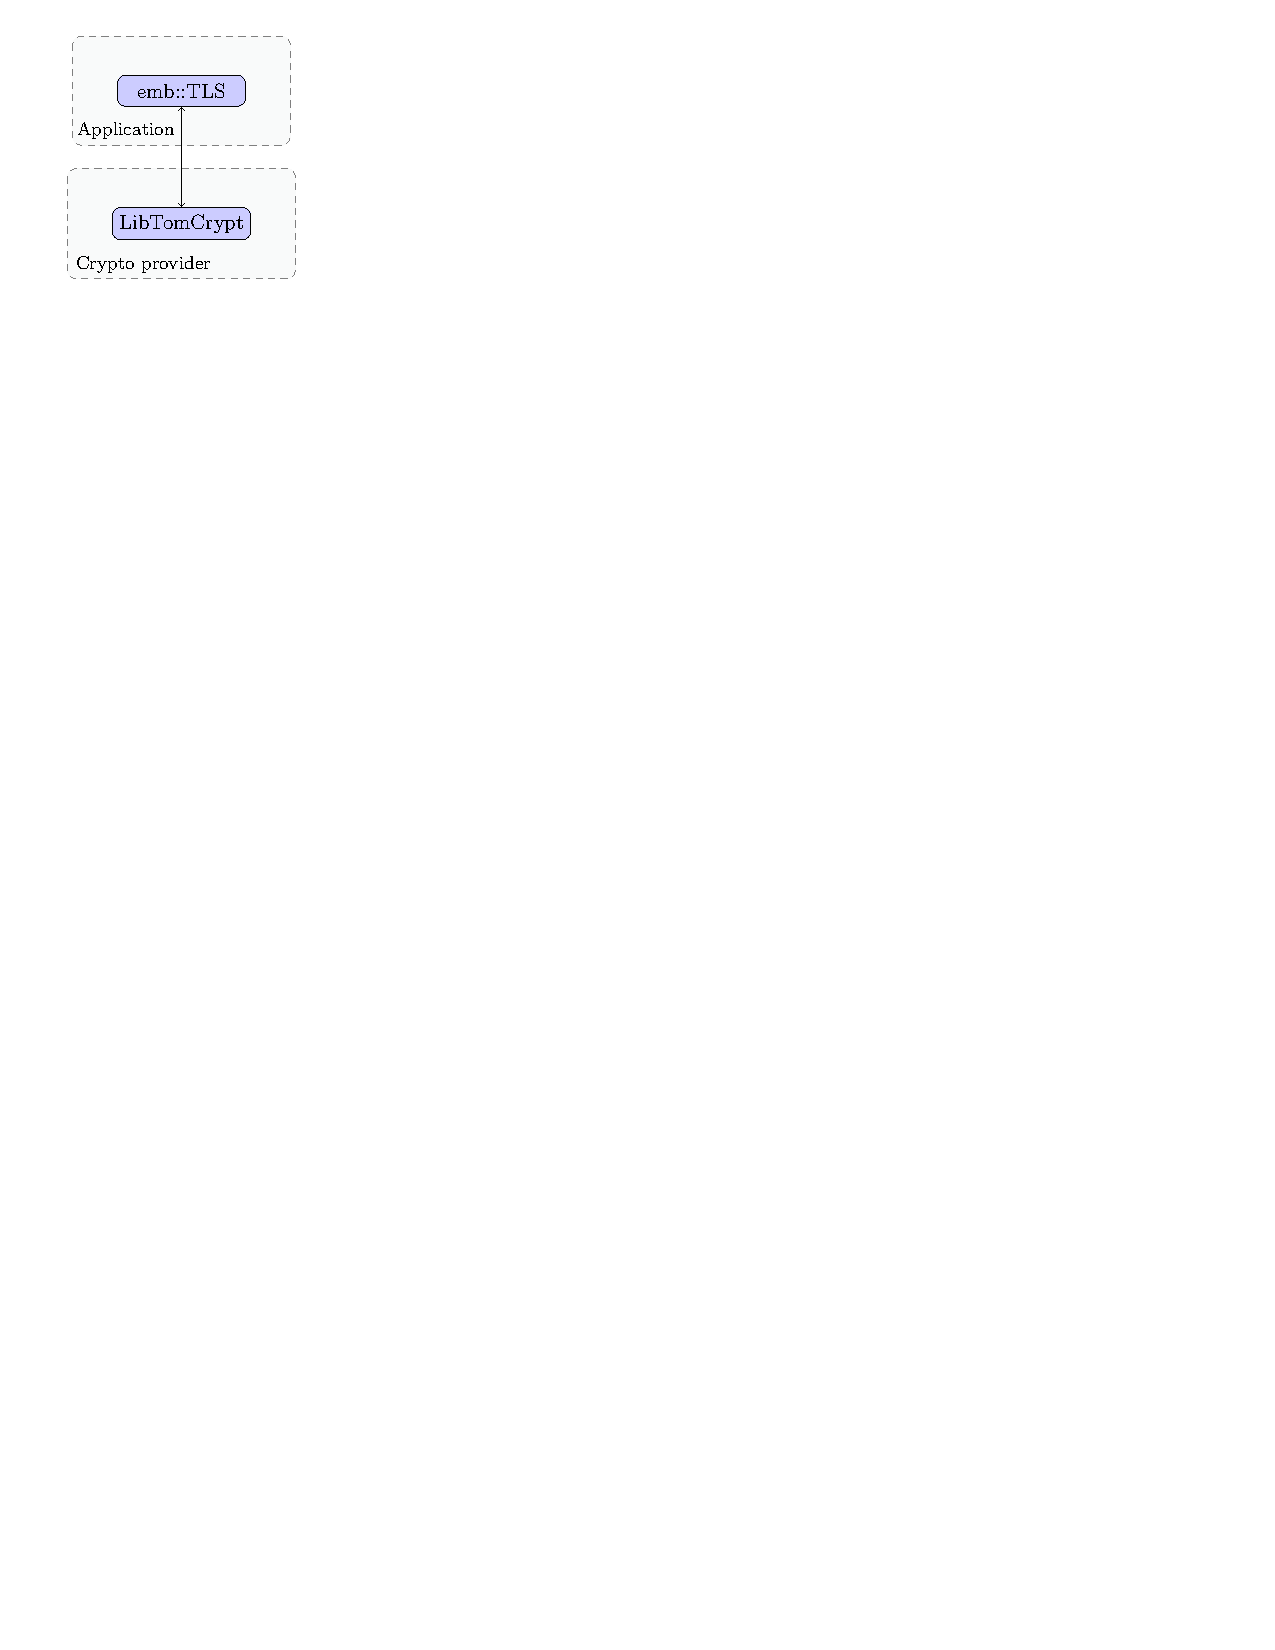
\includegraphics[trim=0cm 23.25cm 15cm 0cm,
height=6.5cm]{figures/intro_embtls.pdf}
\caption{\embtls's project}
\label{fig:motiv_embtls}
%}

\end{figure}
For this, a cryptographic provider (\tomcrypt) is used for the part of
cryptographic calculation needed for the application.
This cryptographic provider is an open-source cryptography software
library.
Problems with this implementation is that only \tomcrypt is
supported as cryptographic providers, meaning that no other libraries can be used
without changing the complete implementation for \embtls.

\begin{figure}[!ht]
\centering
%\frame{
% trim: left, bottom, right, up
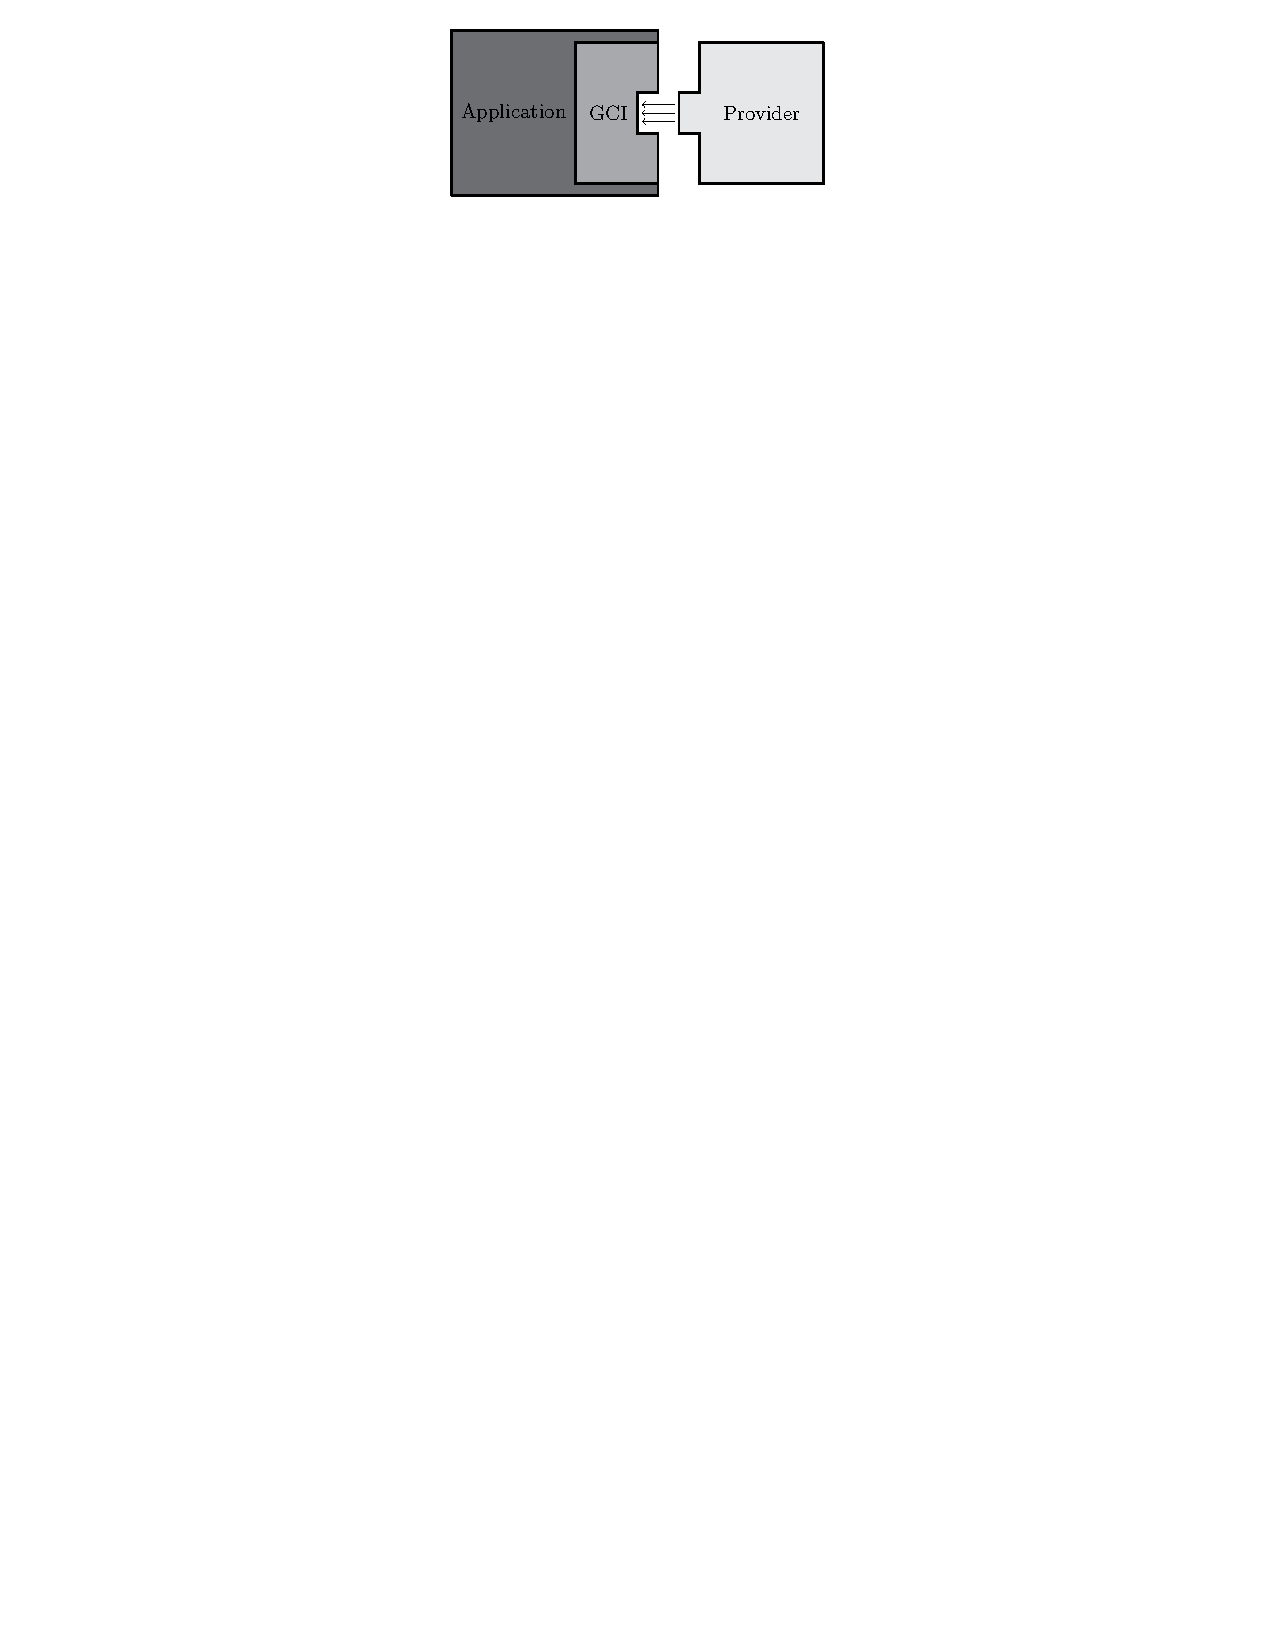
\includegraphics[trim=6cm 24.5cm 2cm 0cm, height=6cm]{figures/intro_gci.pdf}
\caption{Goal of the new implementation}
\label{fig:motiv_gci}
%}
\end{figure}
The goal of the project is therefore to create an interface, a Generic
Cryptographic Interface (GCI), to have a base of the existing cryptography
services and to have the possibility to easily change the providers only by
changing some lines in the interface, instead of the complete
implementation.\newline
Through to this new interface other new cryptographic algorithms may be
easier to add in the interface and to use for the application.\newline
As shown on the figure \ref{fig:motiv_gci}, the interface is implemented in the
application and nothing has to be changed.
The requirements for this Generic Cryptographic Interface (GCI) are listed
below:
\begin{enumerate}
  \item No hidden states shall be used in the interface, meaning that the
  behavior of the cryptographic algorithm functions should only be affected by
  the input parameters.
  All parameters written in input of the function will be used for the
  cryptographic algorithm and nothing else.
  \item Different cryptographic providers may be used for the cryptographic
  calculation. \newline
  That could be open-source cryptographic software libraries or hardware-based cryptographic modules.
  \item With the old version of the implementation (figure
  \ref{fig:motiv_embtls}), the application and the provider interact, meaning
  that when the provider needs informations from the application, this one just send them and
  vice-versa.
  With this new implementation (figure \ref{fig:motiv_gci}) the interface break
  this interaction. To always have this interaction, the interface shall receive
  the information from the application and the provider. These informations
  shall be easily used by both (application and provider) when needed.
\end{enumerate}
 
%\chapter{Design}

%use of context
%work assymetric (do not need the end of a function to begin an other one)
%use of IDs 

\chapter{Generic Cryptographic Interface (GCI)}
As explained in chapter \ref{motiv}, this Generic Cryptographic Interface (GCI)
is implemented in the application and the cryptographic provider shall be easily
changed for another one.
The interface has to be optimized for other projects
too, meaning that it should be as generic as possible. This
interface should have a base of cryptography which can be easily adaptable for
other applications and easily modifiable to use other providers.\newline
Some constraints are added for the interface, which are:
\begin{itemize}
  \item The link between the keys which could come from the application
  and needed in the provider and inversely shall be handled.
  \item No hidden states should be written in the function of the interface,
  meaning that no default parameters for an algorithm has to be written
  internally of a function.\newline
\end{itemize}
In several books and on the internet (see Bibliography) the most
important part of cryptography are listed below:
\begin{itemize}
  \item Hash, which is oft used in signature and MAC algorithms
  \item Signature, which is widely used and also very important
  \item Message Authentication Code (MAC), which has some same properties as
  signatures, but some difference too, which make it important to have it in the
  interface.
  \item Cipher (symmetric and asymmetric), which are needed to encrypt and
  decrypt data
\end{itemize}


\section{Context}
\label{gci_ctx}
%1- what we need
% 2- Explain the solution of the context
As explained above, no hidden states should be written in the function of the
interface, meaning that no default parameters for an algorithm has to be written
internally of a function.
For this constraint the principle of context is used.
Through the context, a configuration of an algorithm can be done, meaning that
in the application part, different parameters for this
algorithm can be chosen and this configuration is saved internally in the
interface (see figure \ref{fig:motiv_gci}).
An ID of where is the configuration saved is returned to the application.\newline
When an update has to be done, the ID is given and the interface knows that the
update has to be done with this configuration.
The cryptographic algorithms which the principle of context is used are:
\begin{itemize}[noitemsep]
  \item Hash algorithm
  \item Signature/MAC algorithm
  \item Cipher algorithm (symmetric and asymmetric)
  \item Diffie-Hellman\newline
\end{itemize}
Through the context, only the parameters added in the configuration are used. No
hidden state is therefore implemented.
The other cryptographic services which don't need a context is because no
configurations are needed to be saved.

\section{Cryptographic services}
\subsection{Hash}
\label{gci_hash}

A hash algorithm is an algorithm which is impossible to compute the input with
the generated output (digest).
It's used in some signature and Message Authentication Code (MAC), that's why is
essential to have it in the interface.
The hash algorithm in the interface is split into three main functions:
\begin{enumerate}[noitemsep]
  \item Configuration of the hash
  \item Update of data
  \item Calculation of the digest
  
\end{enumerate}

\subsection*{Configuration of the hash}

The hash algorithm has only one parameter to be configured, which is which
algorithm should be used for hashing.
The hash algorithm implemented in the interface are:
\begin{itemize}[noitemsep]
  \item MD5
  \item SHA1
  \item SHA224
  \item SHA256
  \item SHA384
  \item SHA512
\end{itemize}

\begin{figure}[!ht]
\centering
%\frame{
% trim: left, bottom, right, up
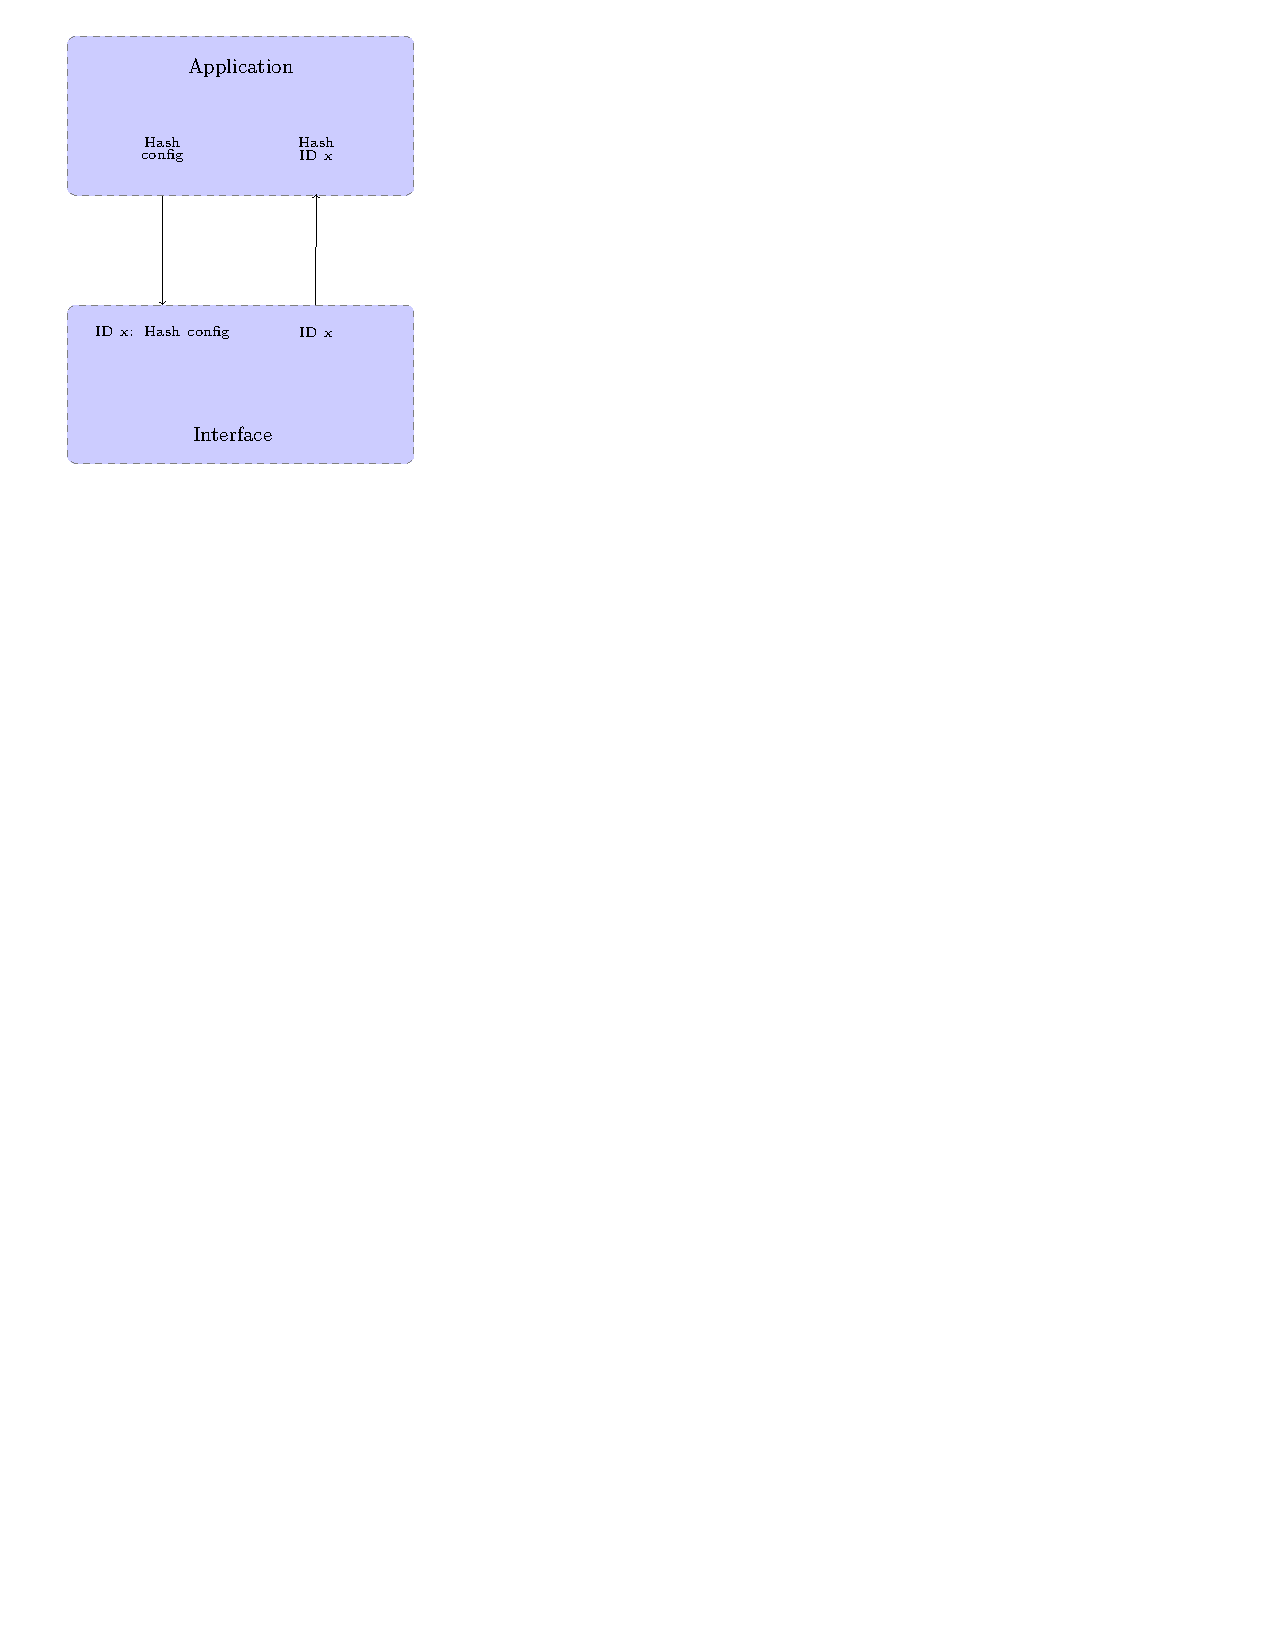
\includegraphics[trim=0cm 20cm 9.5cm 0cm]{figures/hash_example_config.pdf}
\caption{Hash - configuration\newline}
\label{fig:gci_hash_config}
%}
\end{figure}

When the configuration is done this one should be sent to the interface which
will save it in a context.
The interface will then return an ID of the context, which corresponds of
where is saved the configuration.
This is shown on figure \ref{fig:gci_hash_config} 

\subsection*{Update of data}

When the configuration is done, several updates can be done.
The principle on an update is to add a data which we want to hash.

\begin{figure}[!ht]
\centering
%\frame{
% trim: left, bottom, right, up
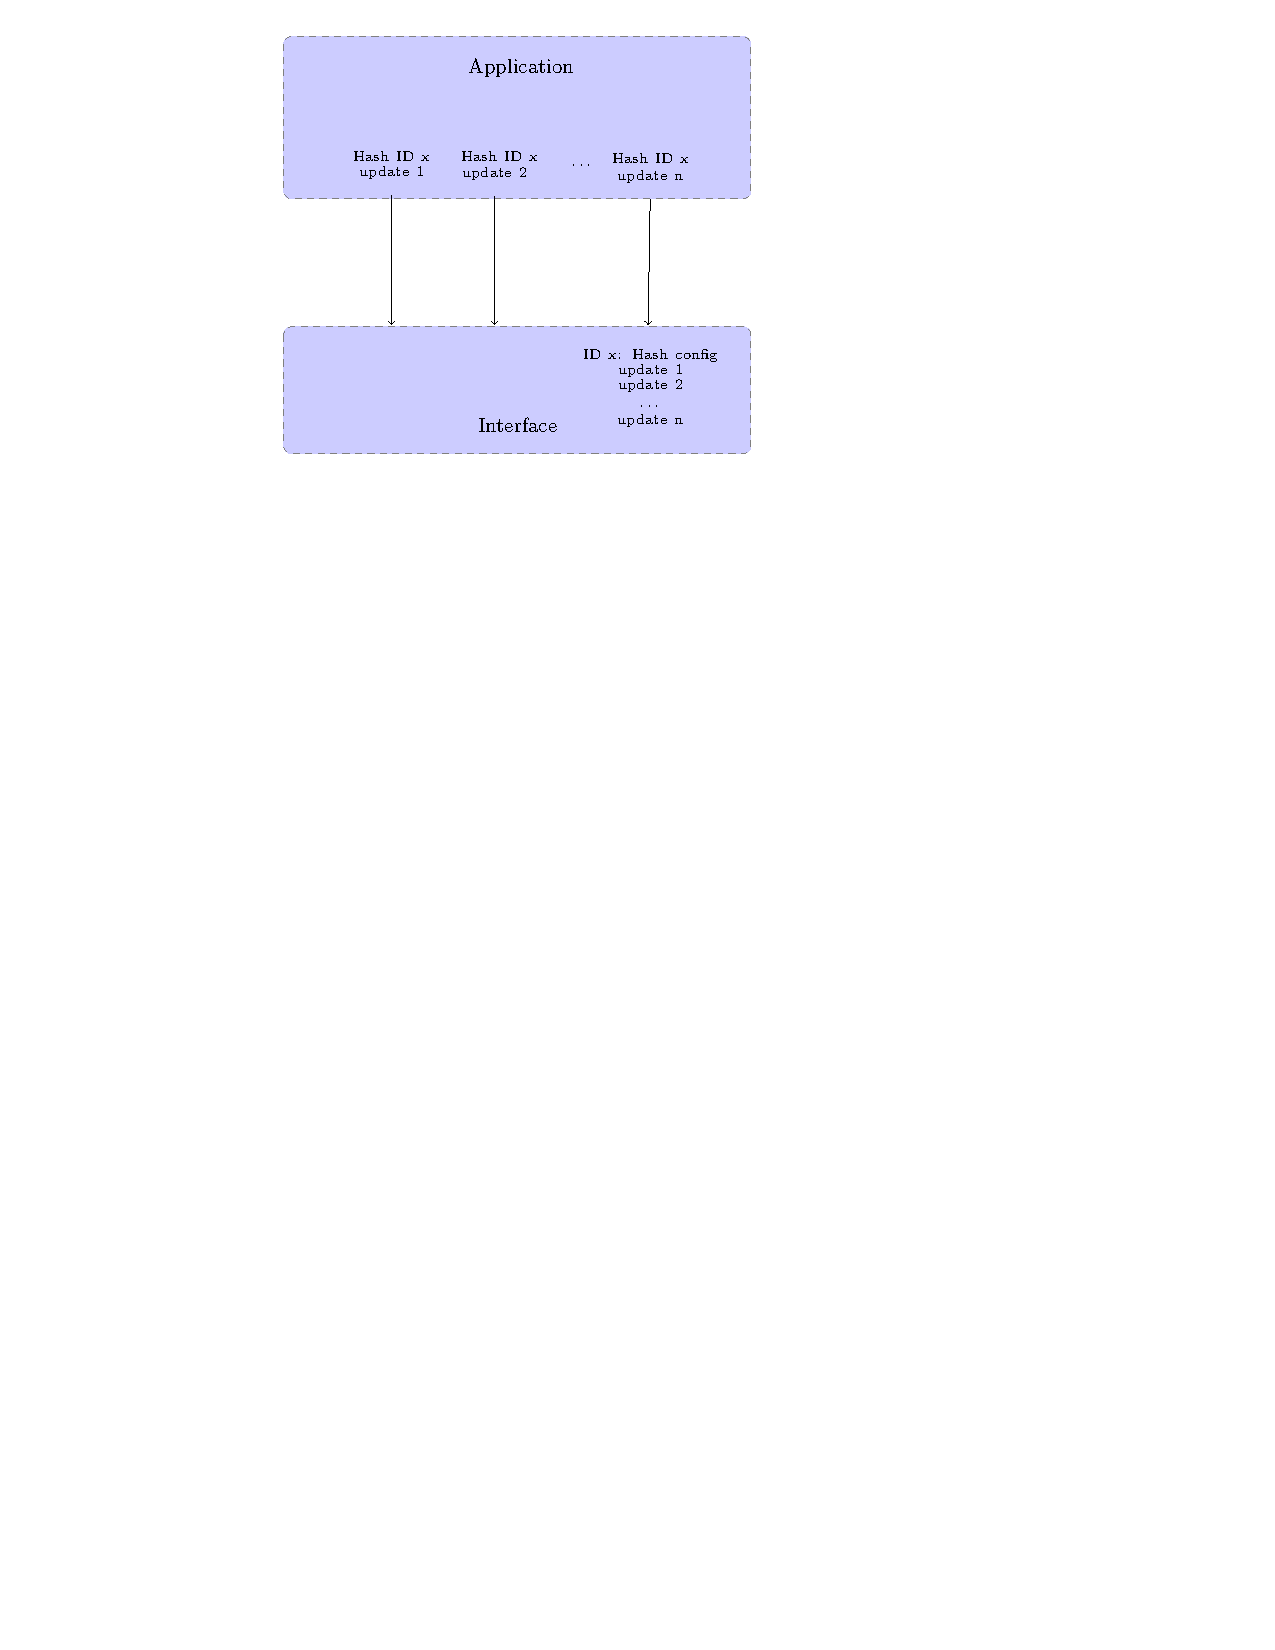
\includegraphics[trim=8cm 20cm 9.5cm 0cm]{figures/hash_example_update.pdf}
\caption{Hash - update\newline}
\label{fig:gci_hash_update}
%}
\end{figure}

As shown in the figure \ref{fig:gci_hash_update}, the ID received in the
configuration part has to be used to add a data.
The ID and the data has therefore sent to the interface, which knows through the
context ID that it should hash the data with the configuration saved in this
context.

\subsection*{Calculation of the digest}

When all the data we want to hash are sent to the interface, the interface can
calculate the digest.

\begin{figure}[!ht]
\centering
%\frame{
% trim: left, bottom, right, up
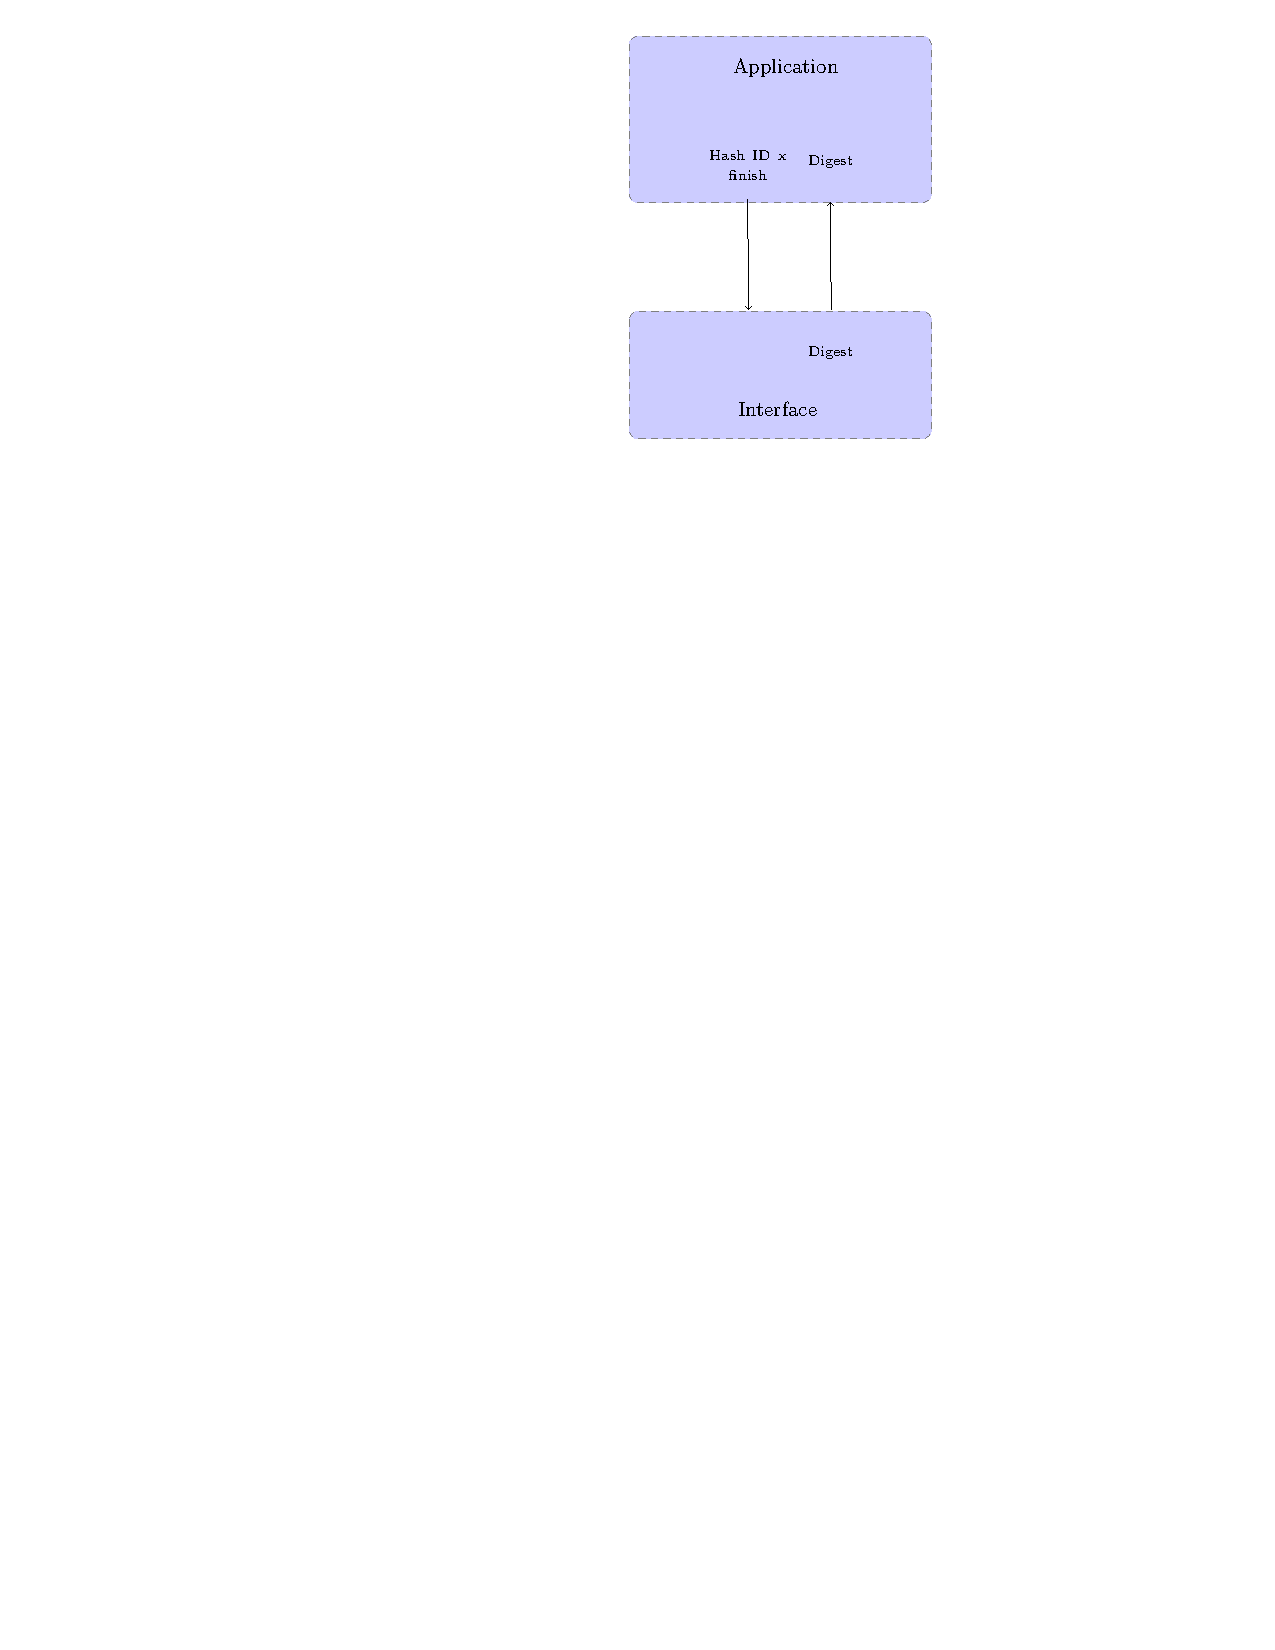
\includegraphics[trim=18.5cm 20cm 9.5cm 0cm]{figures/hash_example_finish.pdf}
\caption{Hash - finish\newline}
\label{fig:gci_hash_finish}
%}
\end{figure}

As shown in figure \ref{fig:gci_hash_finish}, by passing the ID which contains
the configuration and all the updated data, the interface will, through the
provider, calculate the digest.
One of the disadvantages of this part is
when the digest is calculated, all the updated data and the configuration are lost, meaning that we cannot use them
again to calculate another hash with other data.
This problem is solved in chapter \ref{gci_cl_ctx}

\subsection{Generate key pair}
\label{gci_gen_key}

Some parts of cryptography need keys to work, like signatures and ciphers.
The key can be a symmetric, which is the same key for the two peers
in a communication or asymmetric, which is different for the two peers in a
communication.
The goal of this function is to generate the asymmetric keys, public key and
private key. To generate a symmetric key, other methods should be used like
Diffie-Hellman.
In the interface, three kinds of key pair can be generated, each having a
different configuration:
\begin{itemize}
  \item RSA key pair\newline
  The size of the key should be configured (1024 bits, 2048 bits, 4096 bits,
  etc.)
  \item DSA key pair\newline
  The domain parameters can be configured if needed or internally generated
  \item ECDSA key pair (Elliptic curve)\newline
  The type of the elliptic curve should be configured
\end{itemize}

When the configuration is done, this one should be sent to the
interface.
The keys will then be generated through a cryptographic provider.
The keys are, however, returned as IDs, which is one of the principles of the
interface. For more details about the key ID see chapter key management
\ref{gci_key_mng}

\subsection{Digital signature - Message Authentication Code (MAC)}
\label{gci_sign_mac}

The digital signature and the MAC are widely used today. Both provide integrity
and authentication of a message. Only the digital signature provides
non-repudiation more. MAC is much faster than digital signature through the use
of symmetric keys.
As some specifications of certain provider, the signature/MAC function has two
possibilities of use:
\begin{enumerate}[noitemsep]
  \item Signing
  \item Verifying\newline
\end{enumerate}

Each one is split into three functions:
\begin{itemize}[noitemsep]
  \item Configuration of the signature
  \item Update of data
  \item Generate a signature/Verify a signature\newline
\end{itemize}


\subsection*{Configuration of the signature}
For the generation and verification of a signature this part is the same (only
the name of the function changes).
First should the signature be configured.
Several parameters have to be configured which are:
\begin{itemize}
  \item the signature/MAC algorithm, which could be:
  \begin{itemize}[noitemsep]
    \item RSA
    \item DSA
    \item ECDSA
    \item CMAC (MAC from Block Ciphers)
    \item HMAC (MAC from Hash functions)
  \end{itemize}
  \item A hash algorithm, if in the updated data should be first hashed before
  signing, or if the HMAC algorithm is used
  \item The padding, if the RSA algorithm is used
  \item The block mode, the padding and the initialization vector, if the CMAC
  algorithm is used
  \item The private key, if RSA, DSA or ECDSA is used to generate a signature or
  the public key if the same algorithm is used to verify a signature
\end{itemize}

\begin{figure}[!ht]
\centering
%\frame{
% trim: left, bottom, right, up
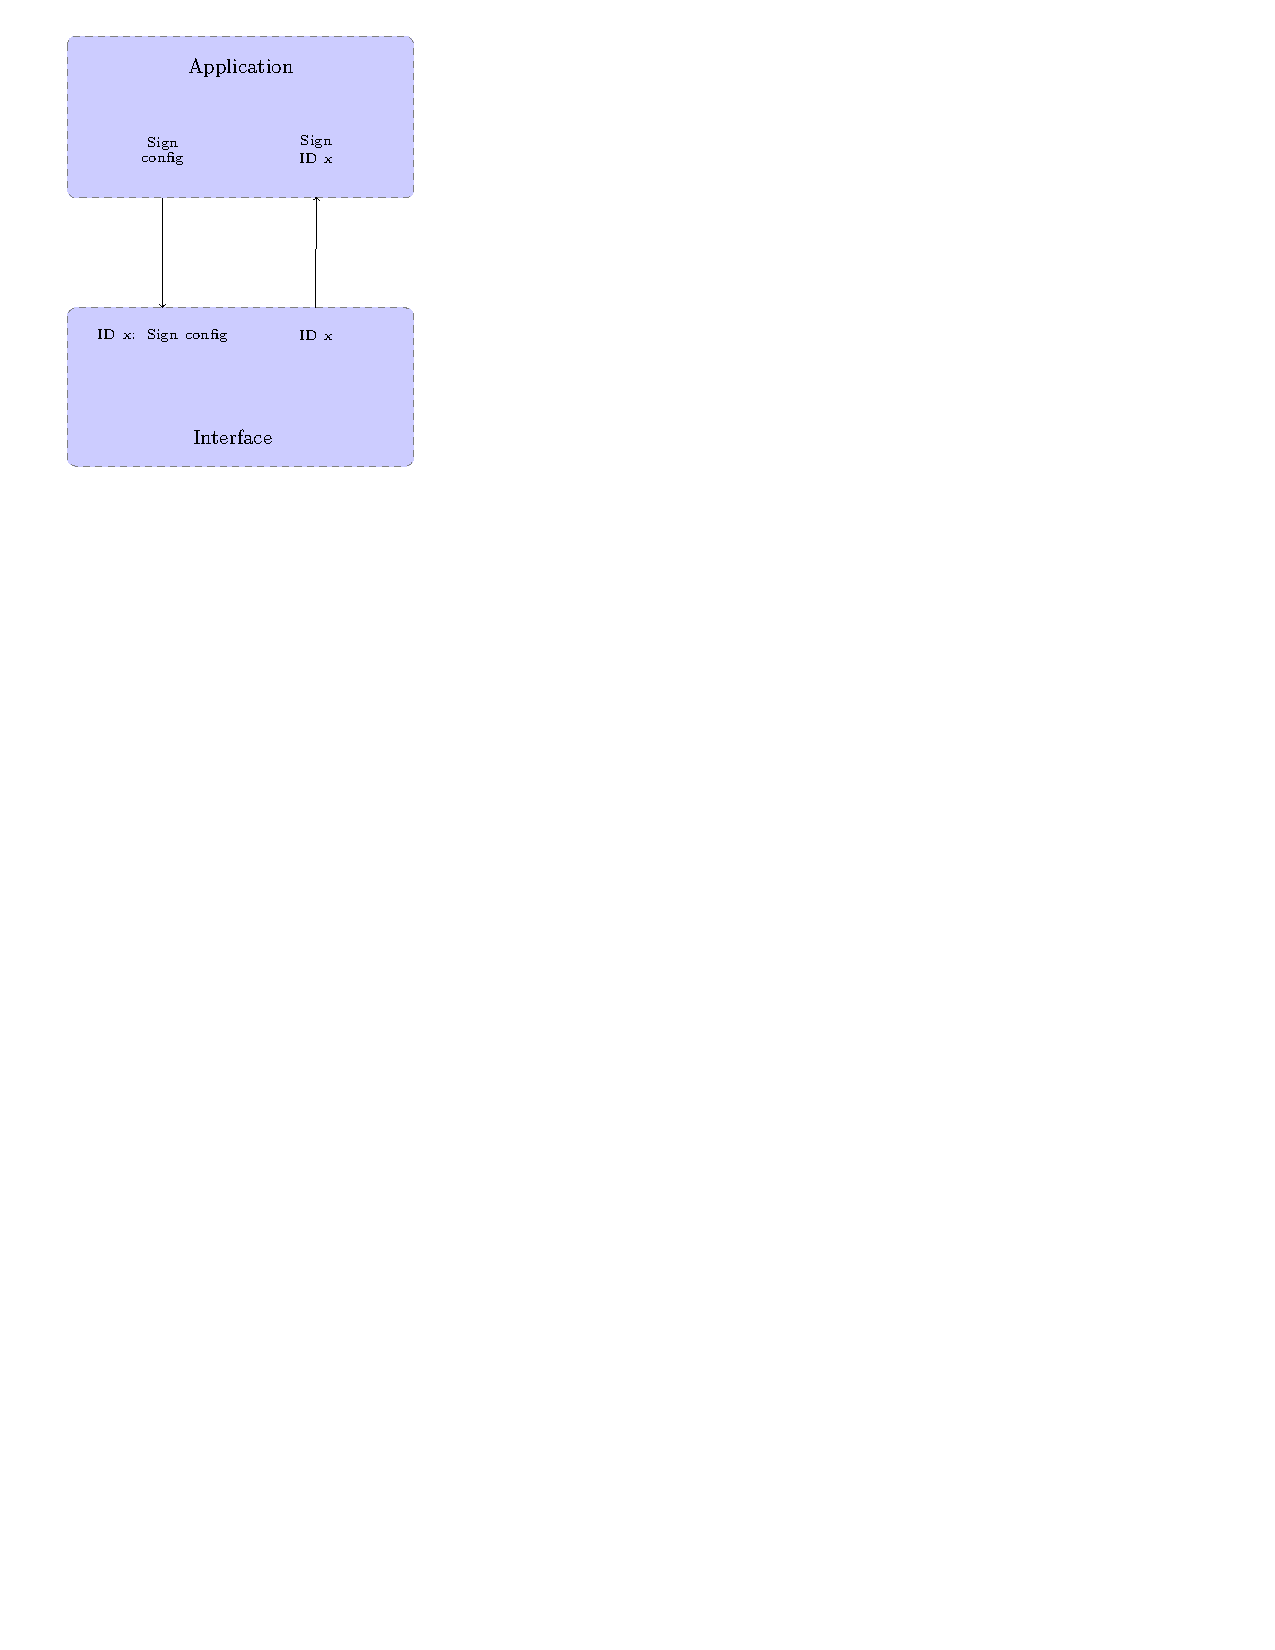
\includegraphics[trim=0cm 20cm 9.5cm 0cm]{figures/sign_example_config.pdf}
\caption{Signature - configuration\newline}
\label{fig:gci_sign_config}
%}
\end{figure}

As shown figure \ref{fig:gci_sign_config}, when the configuration is done, this
one is saved in a context in the interface. An ID of the context is returned,
which indicated where is the configuration saved.

\subsection*{Update of data} 

When the configuration is done, several updates could be done.\newline
The principle of the update is to add data which will be used to generate or
verify a signature.\newline

\begin{figure}[!ht]
\centering
%\frame{
% trim: left, bottom, right, up
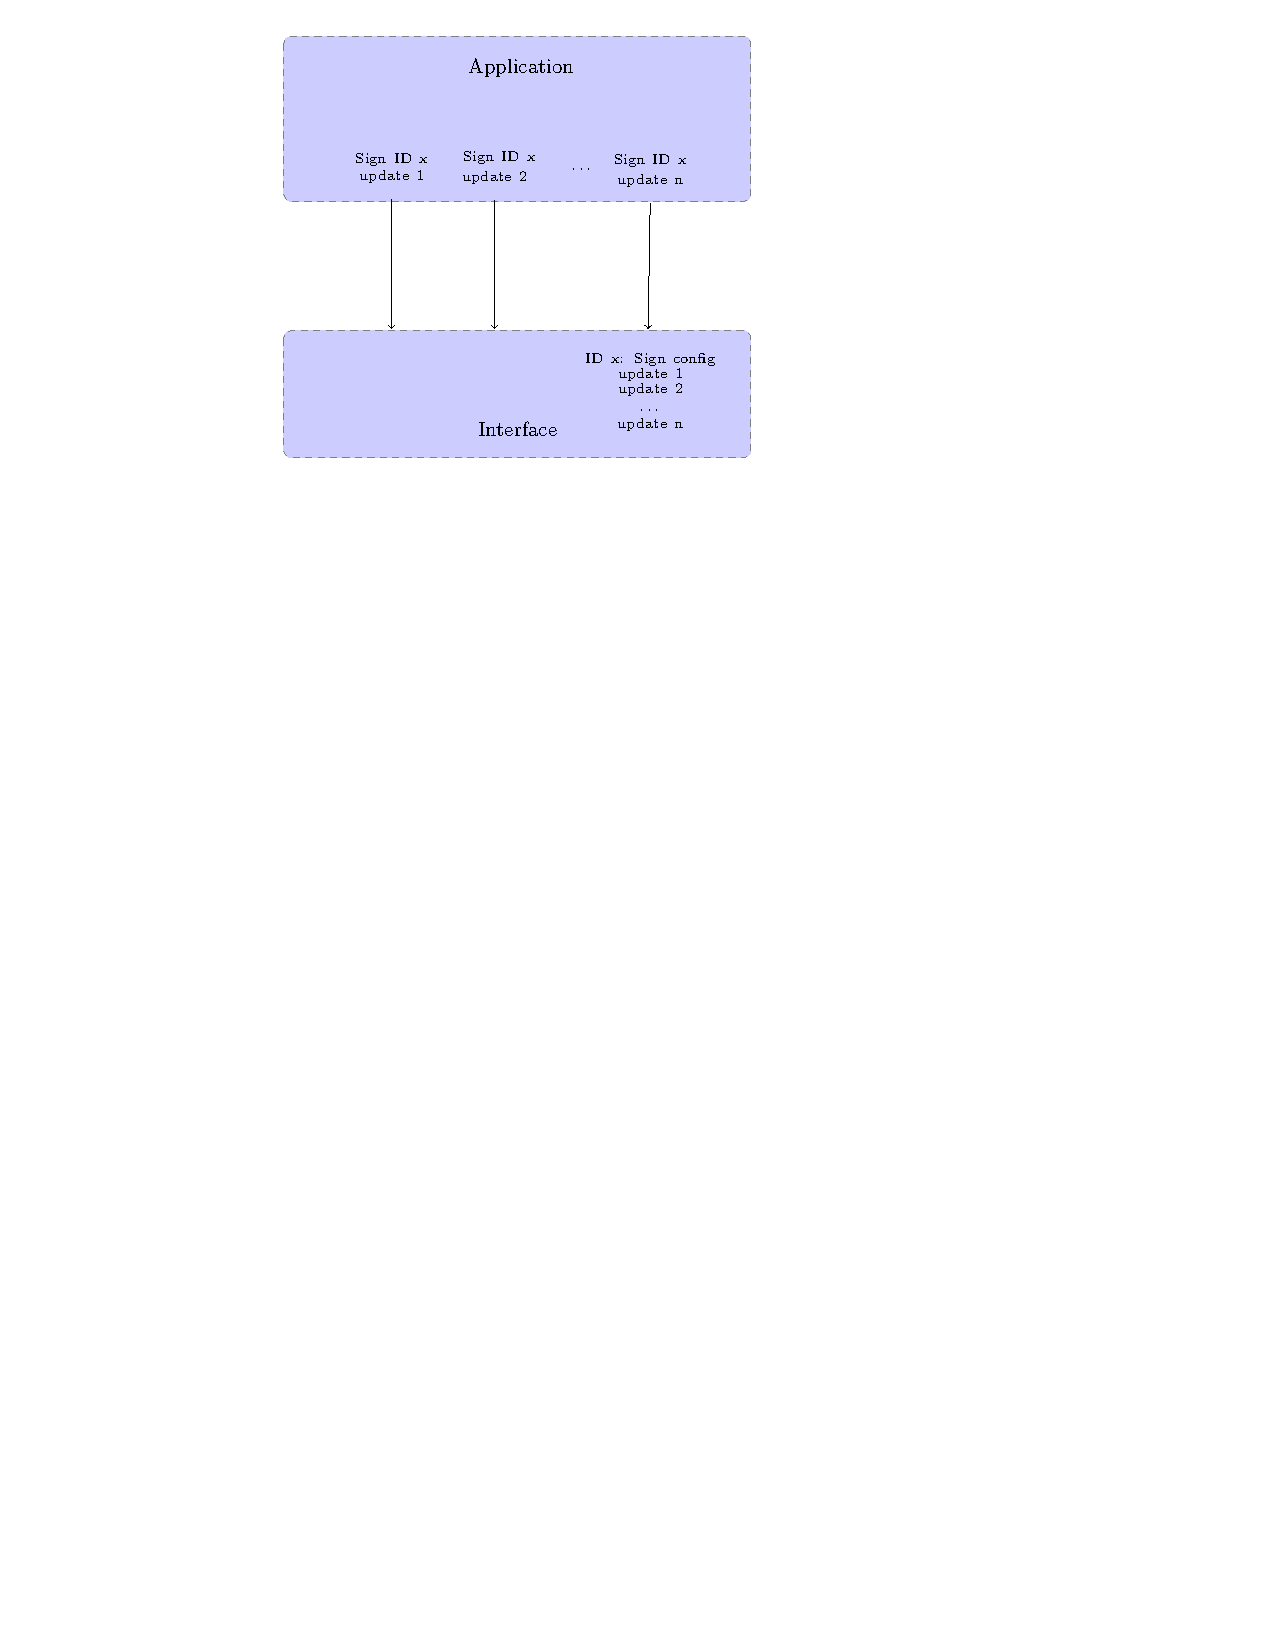
\includegraphics[trim=8cm 20cm 9.5cm 0cm]{figures/sign_example_update.pdf}
\caption{Signature - update\newline}
\label{fig:gci_sign_update}
%}
\end{figure}

As shown in figure \ref{fig:gci_sign_update}, to use the correct configuration,
the ID of the context, returned when the configuration is saved, should be
used.
The data and the ID is then sent to the interface, which will sign this data
with the configuration saved in this context.


\subsection*{Generate a signature/Verify a signature}
\begin{figure}[!ht]
\centering
%\frame{
% trim: left, bottom, right, up
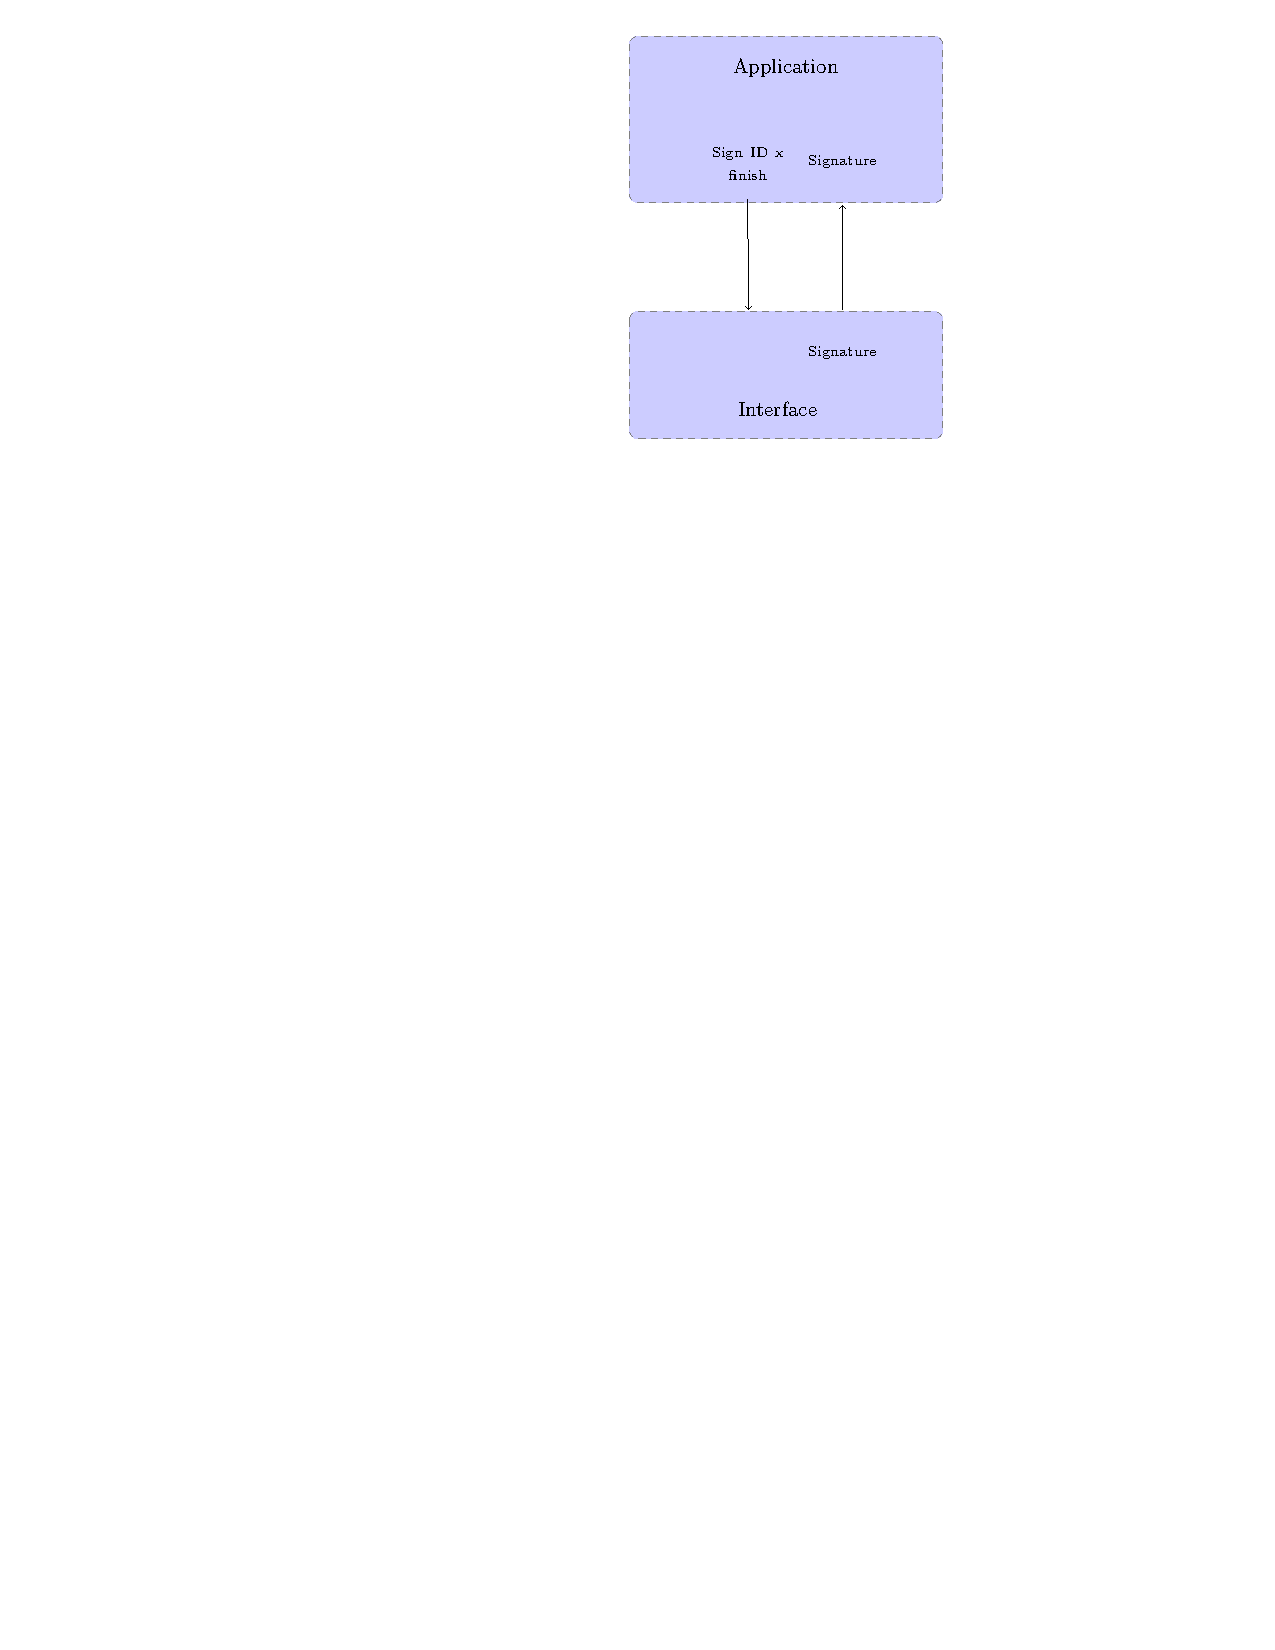
\includegraphics[trim=18.5cm 20cm 9.5cm 0cm]{figures/sign_example_finish.pdf}
\caption{Signature - finish\newline}
\label{fig:gci_sign_finish}
%}
\end{figure}
In this part the generation and the verification are different.
For the generation , the whole updated data and the configuration will be signed
with the private key added in the configuration for the digital
signature but with a symmetric key for the MAC.

For the verification, the signature we want to verify should be added to the
function.
Then the updated data will be signed, but with the public key for the
digital signature, and the same symmetric key as the generation of the
signature for the MAC.
Then the added signature (which is done with the
private key) could be compared with the ``signature'' computed to verify.
The most important part of the verification is that the private key, which
the signature is done and the public key for the verification, should be
generated together for the digital signature and the same symmetric key should
be used for the MAC.

\subsection{Cipher (symmetric and asymmetric)}
\label{gci_ciph}
A cipher, as explained in \ref{intro_cipher}, which
could be symmetric or asymmetric, is an algorithm for encrypting and decrypting
data.
This concept is therefore used in the interface and split into three main
functions which are:
\begin{itemize}[noitemsep]
  \item Configuration of the cipher
  \item Encryption of a plaintext
  \item Decryption of a ciphertext
\end{itemize}

\subsection*{Configuration of the cipher}
Several parameters are to be configured for the cipher algorithm and depends
particularly of which cipher algorithm is used.
The cipher algorithm is split into three main algorithm:

\begin{itemize}
  \item Symmetric stream cipher algorithm\newline
Today very deprecated but is, however, implemented in the interface if
comparison has to be done.
Only the RC4 stream cipher is implemented in the interface.
Other stream ciphers can, however, be easily added in the interface if
needed.
Nothing more as the algorithm has to be configured for the use of
it.
  \item Symmetric block cipher algorithm\newline
  Three kinds of symmetric block cipher algorithms are used today and
therefore implemented in the interface:
\begin{itemize}[noitemsep]
  \item Data Encryption Standard (DES)
  \item 3DES, three subsequent DES encryption
  \item Advanced Encryption Standard (AES)  
\end{itemize}
Each symmetric block cipher algorithm needs a mode of operation, named block
mode in the interface, which depends on the size of data we want to
encrypt.\newline
The block modes implemented in the interface are:
\begin{itemize}[noitemsep]
  \item Electronic Code Book mode (ECB)
  \item Cipher Block Chaining mode (CBC)
  \item Cipher Feedback mode (CFB)
  \item Output Feedback mode (OFB)
  \item Counter mode (CTR)
  \item Galois Counter Mode (GCM)
\end{itemize}
  \item Asymmetric algorithm\newline
  Only the RSA algorithm is implemented for this part of the interface.
  In practice to use the RSA algorithm this one should use a padding to increase
  the security of it.
  The best known padding in the Public-Key Cryptography Standard (PKCS) and is,
of course, implemented in the interface.\newline  
\end{itemize} 
The most important thing for a cipher is, of course, the key!
For a symmetric cipher, stream or block, the key is only a shared key.
For an asymmetric cipher, if an encryption will be done, a public key should
be added. If a decryption will be done, a private key should be added to the
configuration.

\begin{figure}[!ht]
\centering
%\frame{
% trim: left, bottom, right, up
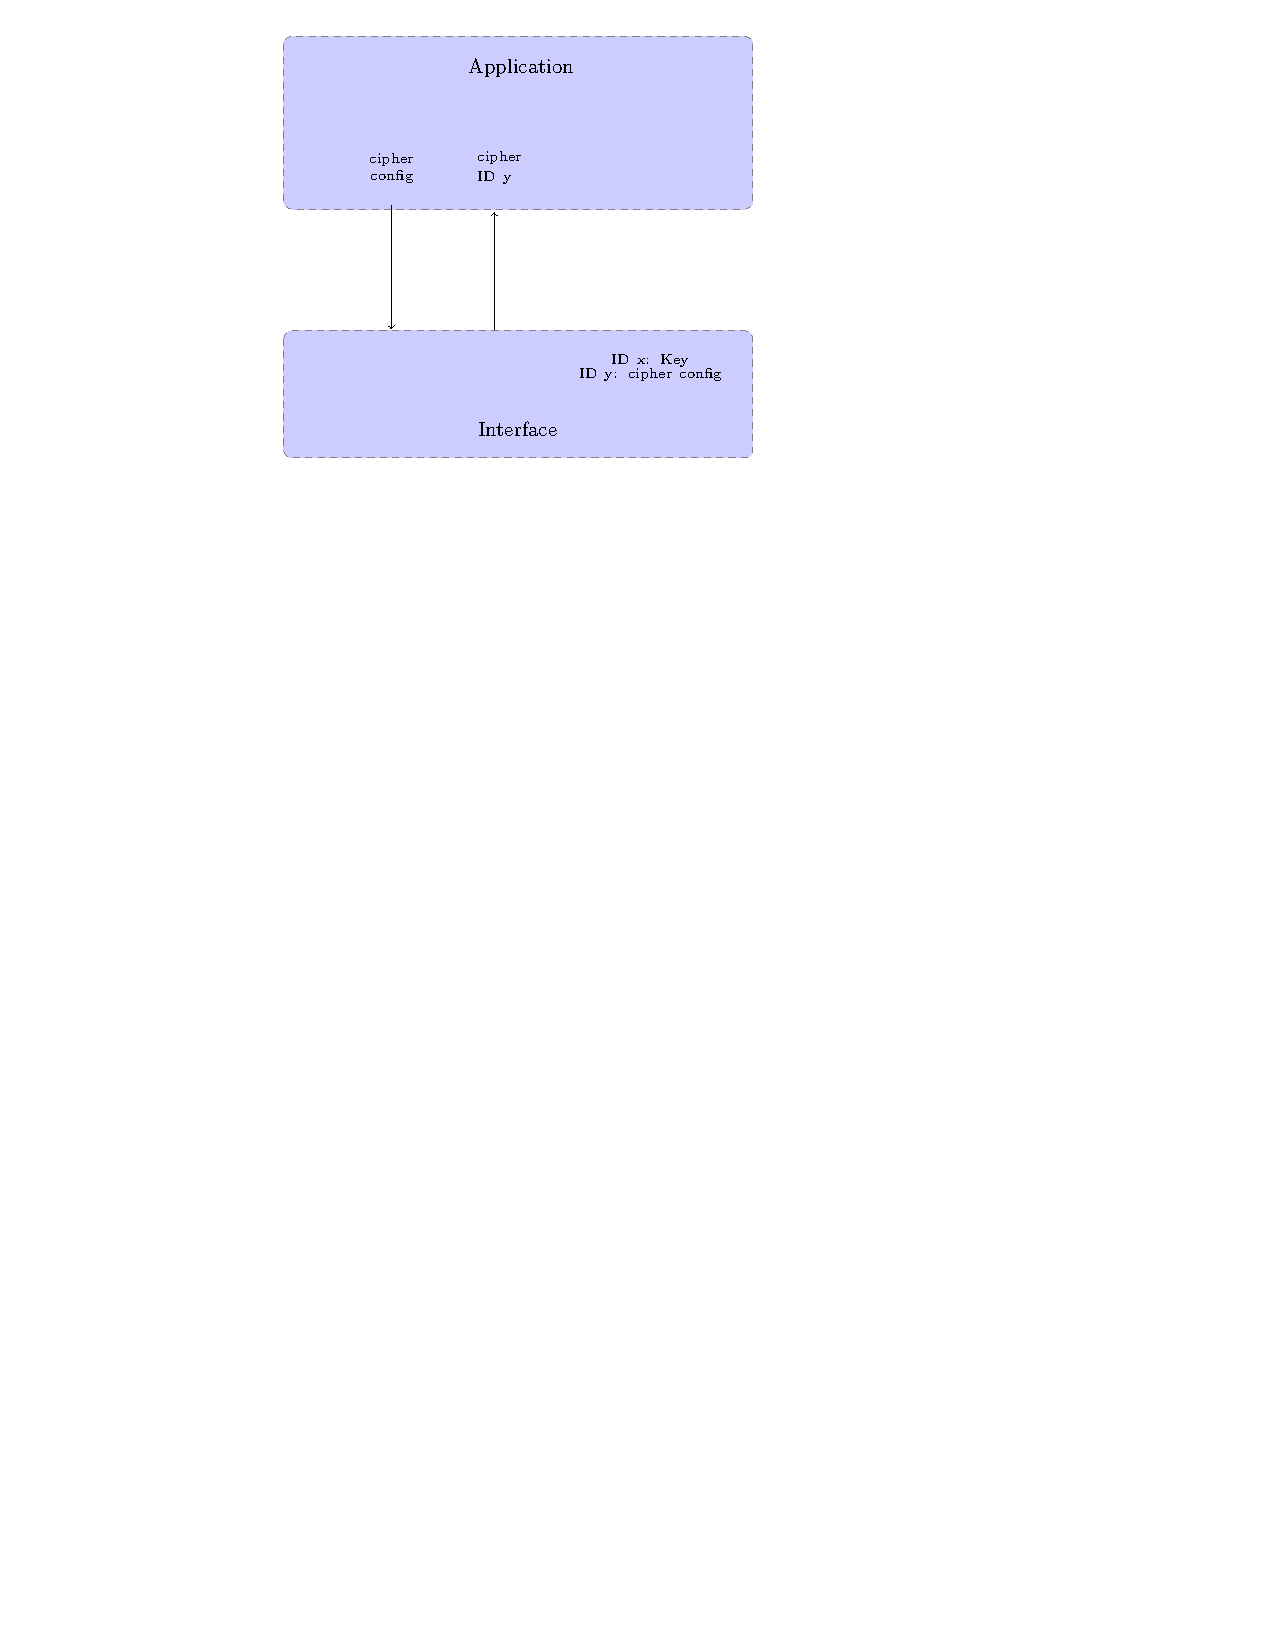
\includegraphics[trim=8.5cm 20cm 9.5cm 0cm]{figures/cipher_example_config.pdf}
\caption{Cipher - configuration\newline}
\label{fig:gci_cipher_config}
%}
\end{figure}

When the configuration is done this one should be sent to the interface
which will save it in a context.
The interface returned an ID of the context, which corresponds of where is saved
the configuration if this one should be used in the future.
The key added to the function is an ID of the key which is already saved in
the interface.
This principle is shown in figure \ref{fig:gci_cipher_config}

\subsection*{Encryption of a plaintext}
\begin{figure}[!ht]
\centering
%\frame{
% trim: left, bottom, right, up
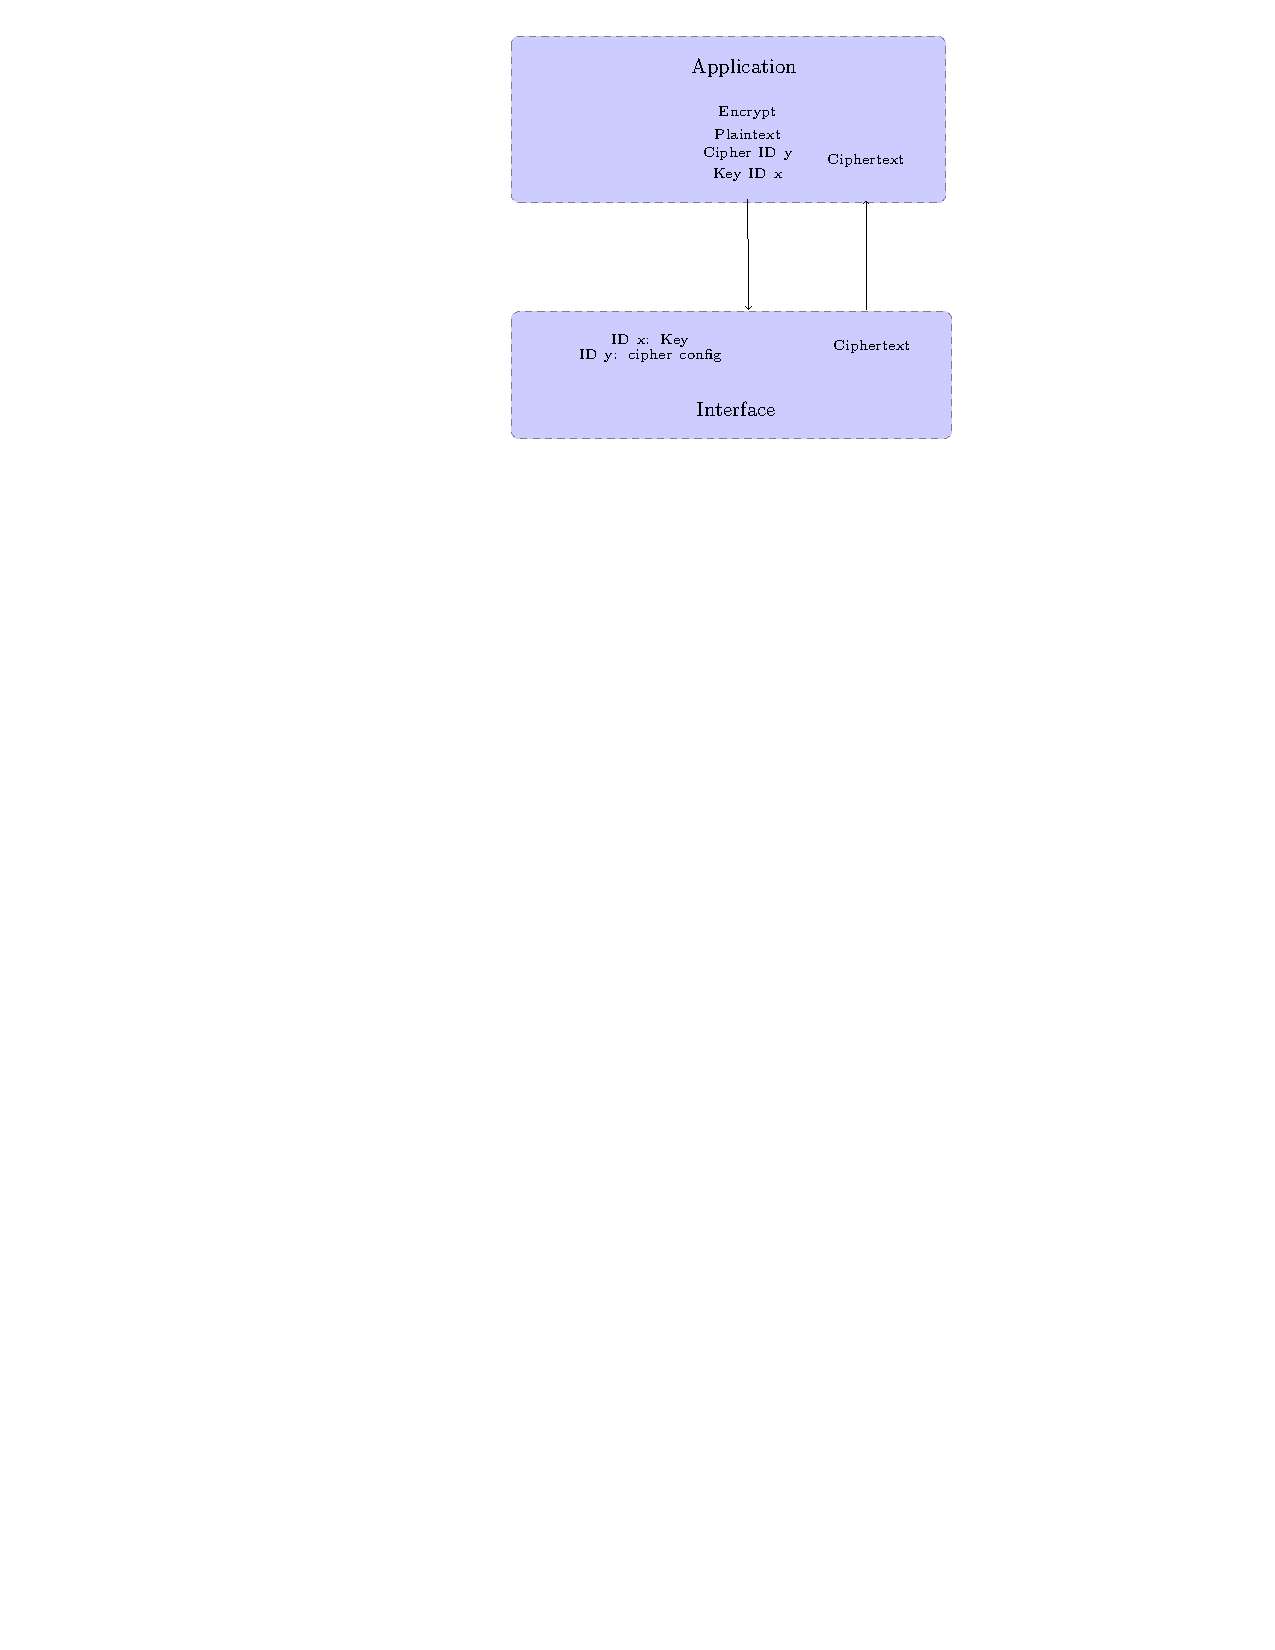
\includegraphics[trim=16cm 20cm 9.5cm 0cm]{figures/cipher_encrypt.pdf}
\caption{Cipher - Encryption\newline}
\label{fig:gci_cipher_encrypt}
%}
\end{figure}
When the configuration is done, a encryption can be done.
To encrypt data, the ID of the context (where is the configuration saved)
should be added to the function with the data to encrypt (plaintext).
The interface will, through a provider, calculate the ciphertext of the
plaintext with the configuration saved previously in the context.
This principle is shown figure \ref{fig:gci_cipher_encrypt}


\subsection*{Decryption of a ciphertext}

\begin{figure}[!ht]
\centering
%\frame{
% trim: left, bottom, right, up
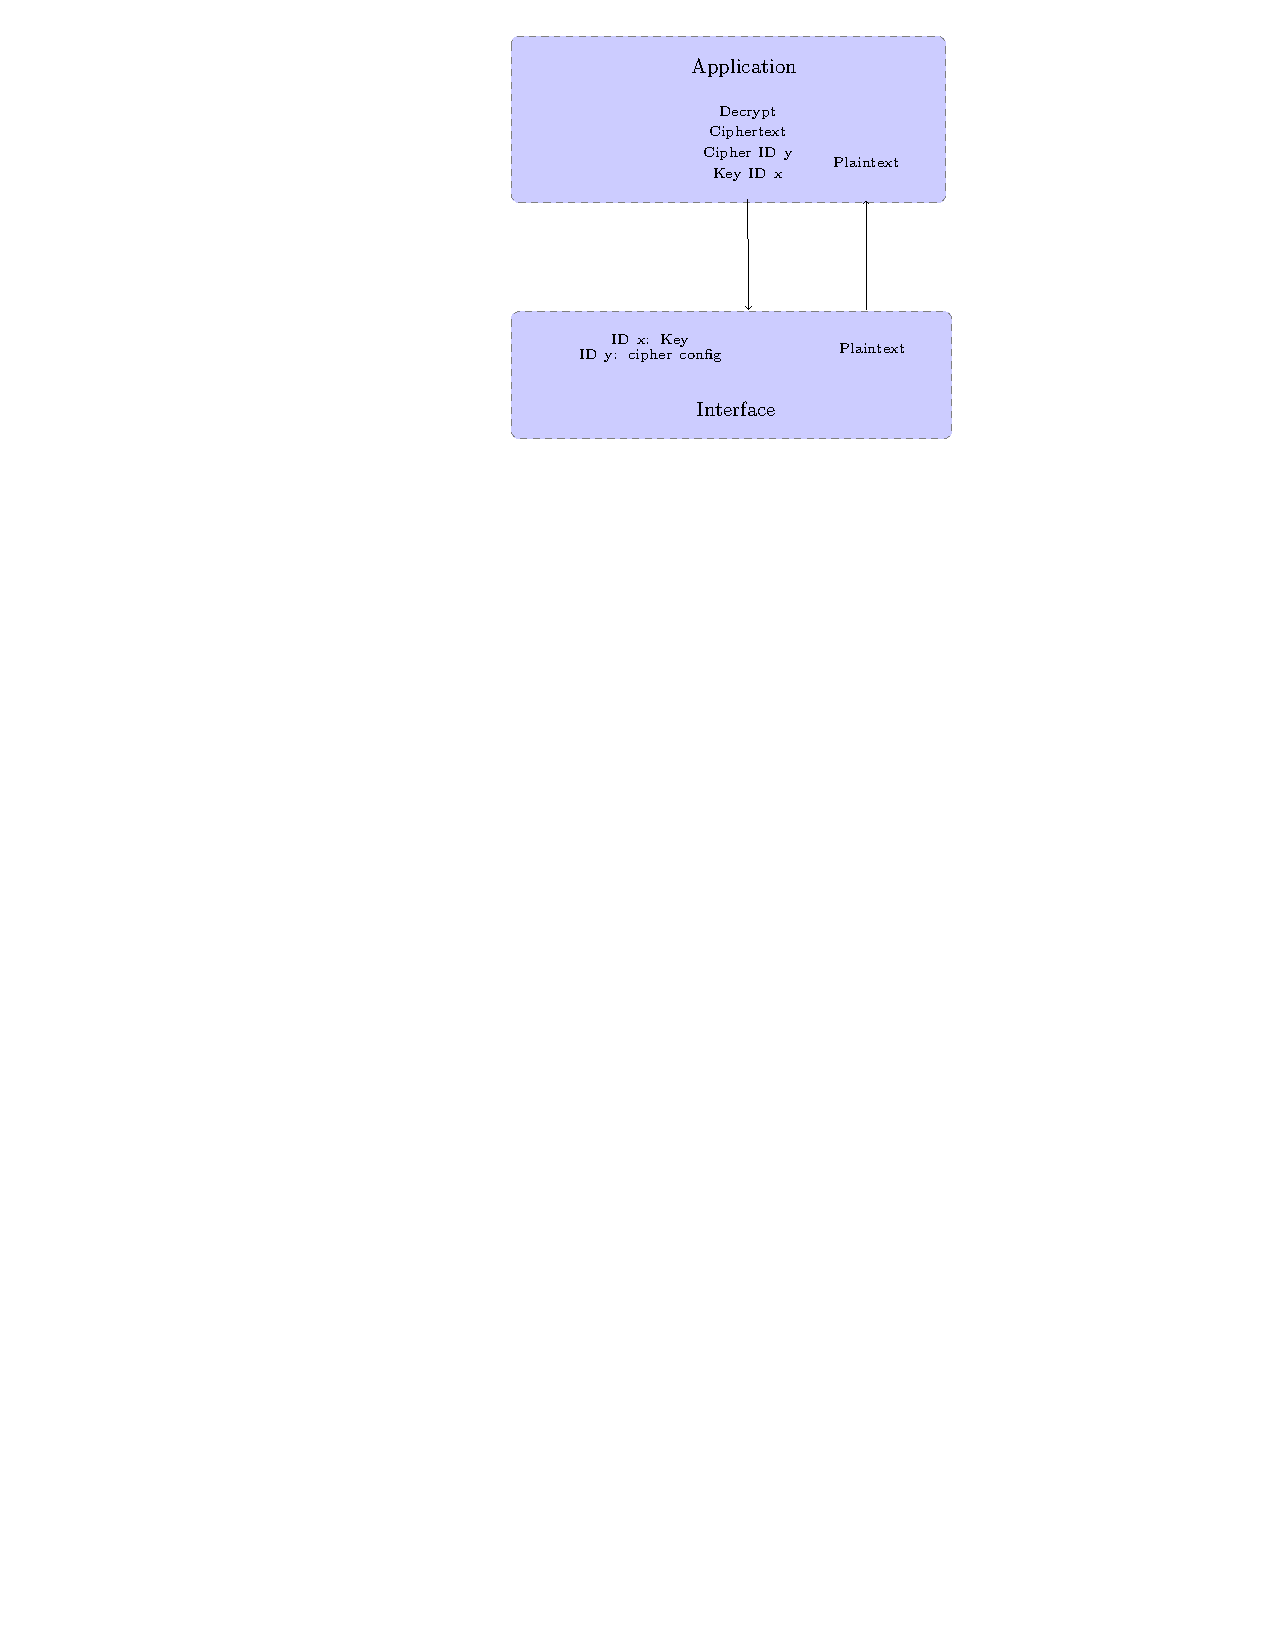
\includegraphics[trim=16cm 20cm 9.5cm 0cm]{figures/cipher_decrypt.pdf}
\caption{Cipher - Decryption\newline}
\label{fig:gci_cipher_decrypt}
%}
\end{figure}
When the configuration is done, a decryption can be done.
To decrypt a data, the ID of the context (where is the configuration saved)
should be added to the function with the data to decrypt (ciphertext).
The interface will, through a provider, calculate the plaintext of the
ciphertext with the configuration saved previously in the context.
This principle is shown figure \ref{fig:gci_cipher_decrypt}


\subsection{Diffie-Hellman}
\label{gci_dh}

Diffie-Hellman key exchange is a specific method of securely exchanging
cryptographic keys over an insecure network. It starts with asymmetric keys to finish with a
symmetric, shared key which is the same for the two peer in a communication.

The Diffie-Hellman key exchange should therefore have the possibility to
generate key pairs and to calculate the shared key.

That's why in the interface the Diffie-Hellman protocol is split into three main
functions:
\begin{itemize}[noitemsep]
  \item Configuration of the Diffie-Hellman protocol
  \item Generation key pair
  \item Calculation of the shared key
\end{itemize}


\subsubsection*{Configuration of the Diffie-Hellman protocol}
The Diffie-Hellman key exchange and the Elliptic Curve of Diffie-Hellman key
exchange can be used in the interface.
For the configuration, one of these key exchanges should be chosen.

For the Diffie-Hellman key exchange the domain parameters can be added. If no
domain parameters have been added, the interface will, through the provider,
generate them.

For the Elliptic Curve of Diffie-Hellman key exchange, the type of curve should
be configured.

\begin{figure}[!ht]
\centering
%\frame{
% trim: left, bottom, right, up
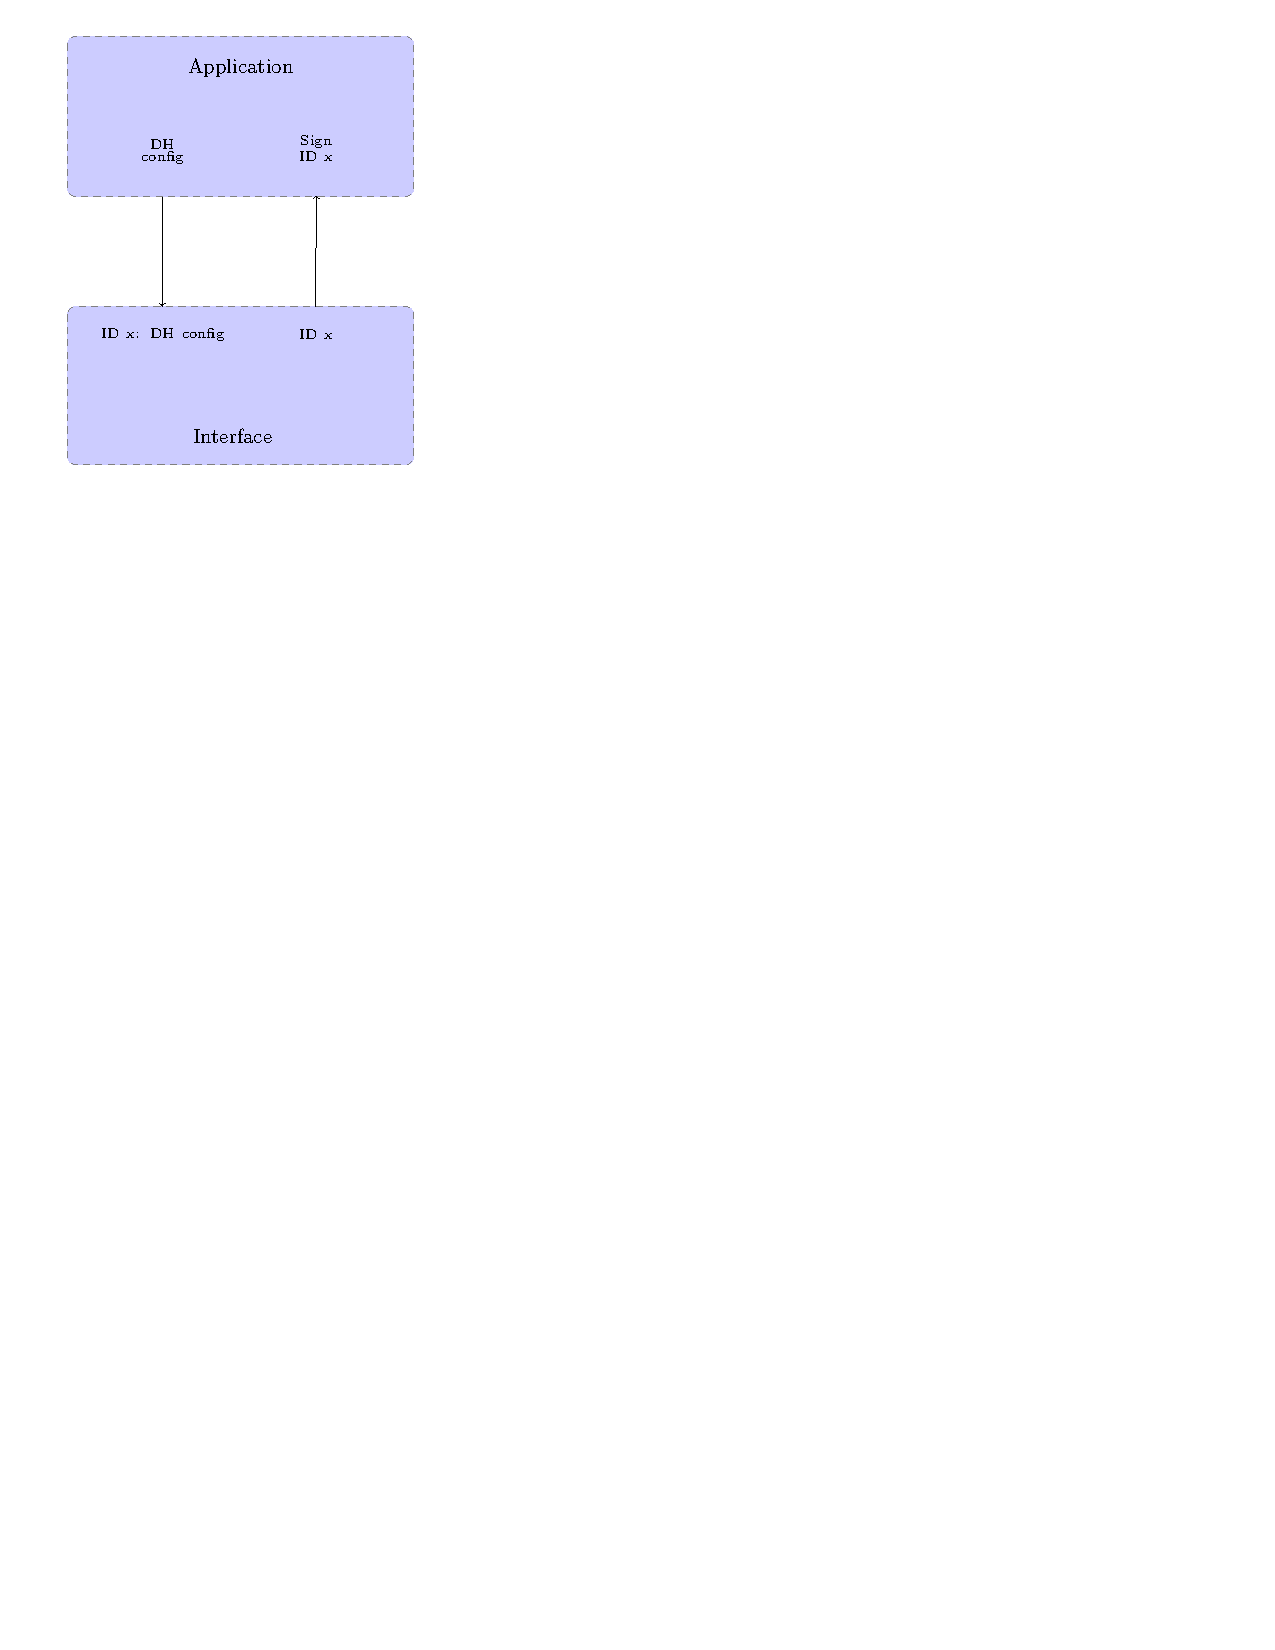
\includegraphics[trim=0cm 20cm 10cm 0cm]{figures/gci_dh_config.pdf}
\caption{DH - Configuration\newline}
\label{fig:gci_dh_config}
%}
\end{figure}

As shown on figure \ref{fig:gci_dh_config}, when the configuration is done, this
one should be sent to the interface which will save it in a context.
An ID of the context will be returned to the application, which indicates the
placement of the context, also of the configuration.


\subsubsection*{Generation of the key pair}

When the configuration is done, key pair can be generated. It's the same
principle as explain in the chapter \ref{gci_gen_key}, but for the
Diffie-Hellman it's a little bit different. The private key of the Diffie must not go out of the
interface. That's why when the key should be generated only the ID of the public
key will go out of the function. The private key will be saved in the
context, same context where is the configuration saved. This is why
Diffie-Hellman is not implemented with the asymmetric cipher algorithm, where
the public key and private key are going out of the function and don't stay in
the context. This is shown on figure \ref{fig:gci_dh_gen_key}

\begin{figure}[!ht]
\centering
%\frame{
% trim: left, bottom, right, up
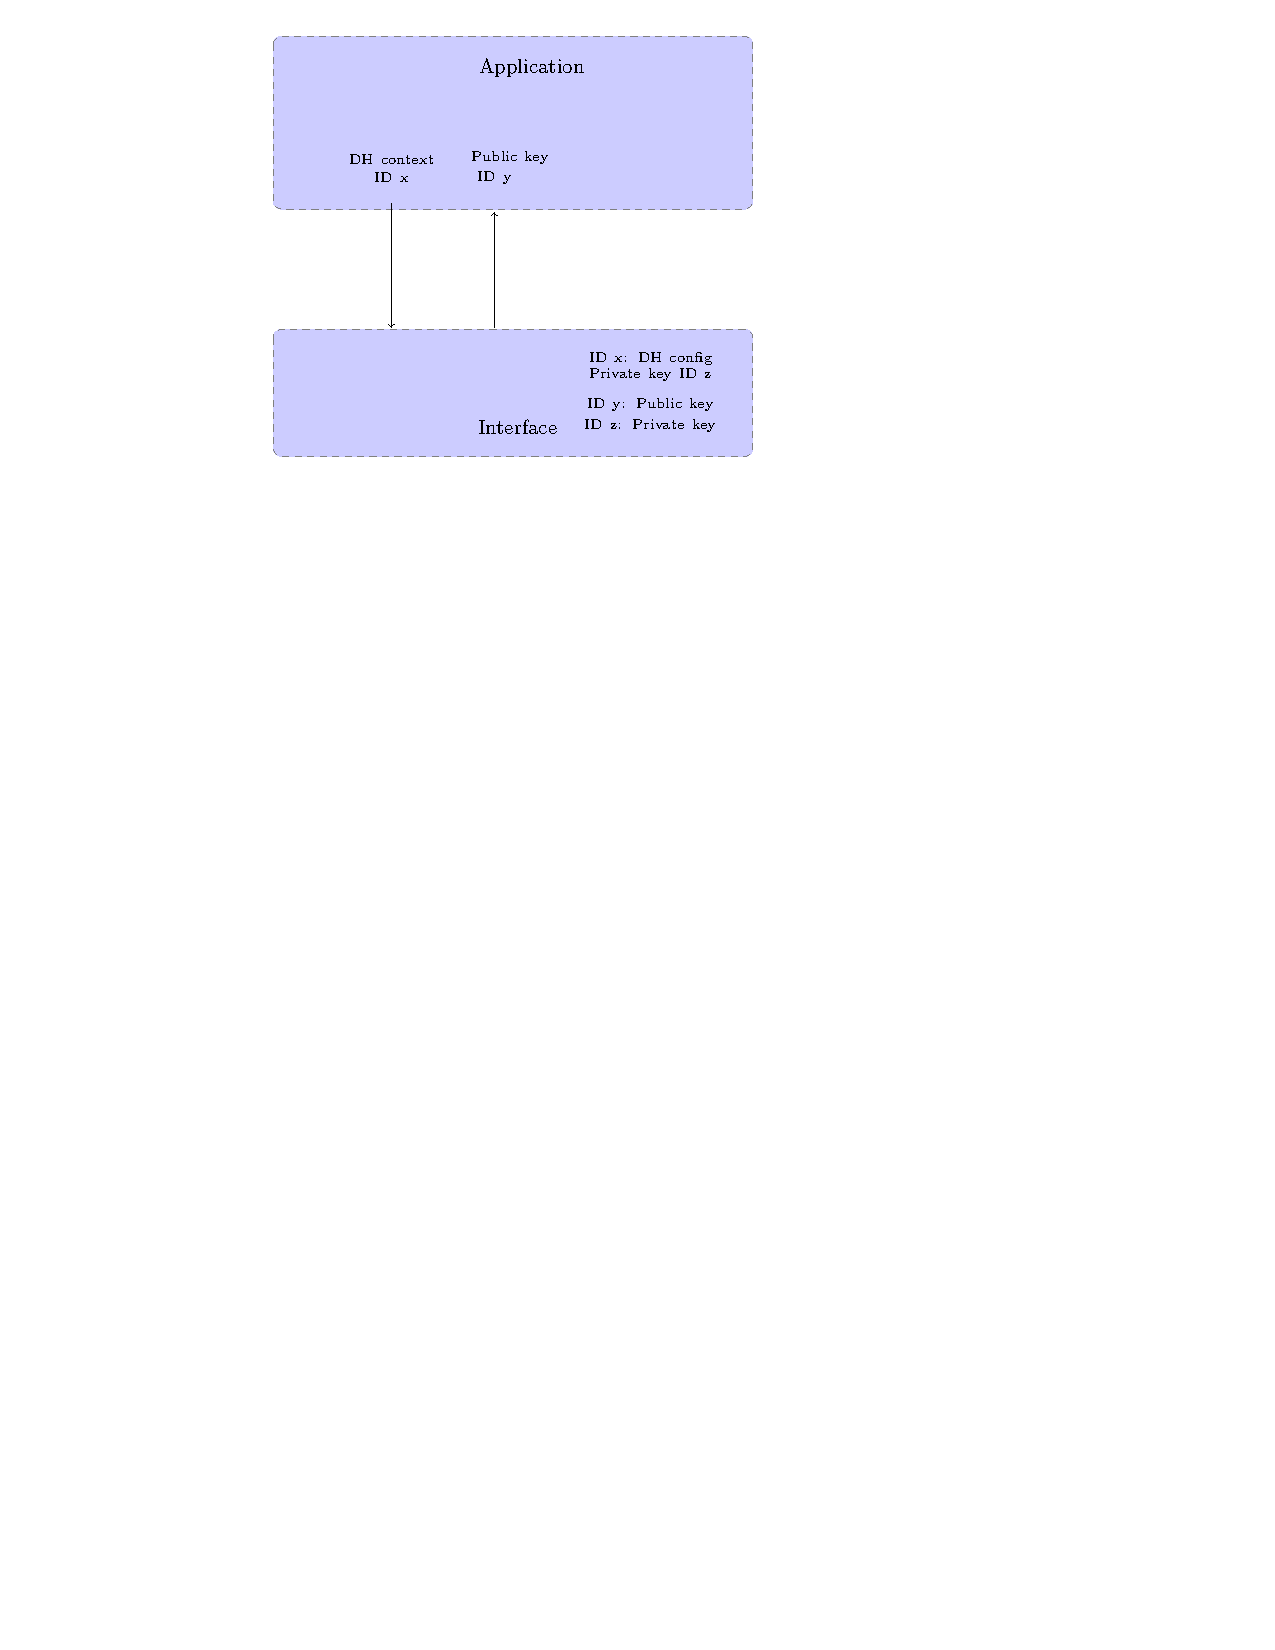
\includegraphics[trim=8.5cm 20cm 10cm 0cm]{figures/gci_dh_gen_key.pdf}
\caption{Diffie-Hellman - Generate key pair\newline}
\label{fig:gci_dh_gen_key}
%}
\end{figure}


\subsubsection*{Calculation of the shared key}

When the public key of the peer is received, the shared key could be generated.
To do it, the context with the configuration and the private, and the public key
of the peer should be added to the interface. This one will, through a provider
calculate the shared key and returned the ID of this one. This is shown on
figure \ref{fig:gci_dh_calc_key}

\begin{figure}[!ht]
\centering
%\frame{
% trim: left, bottom, right, up
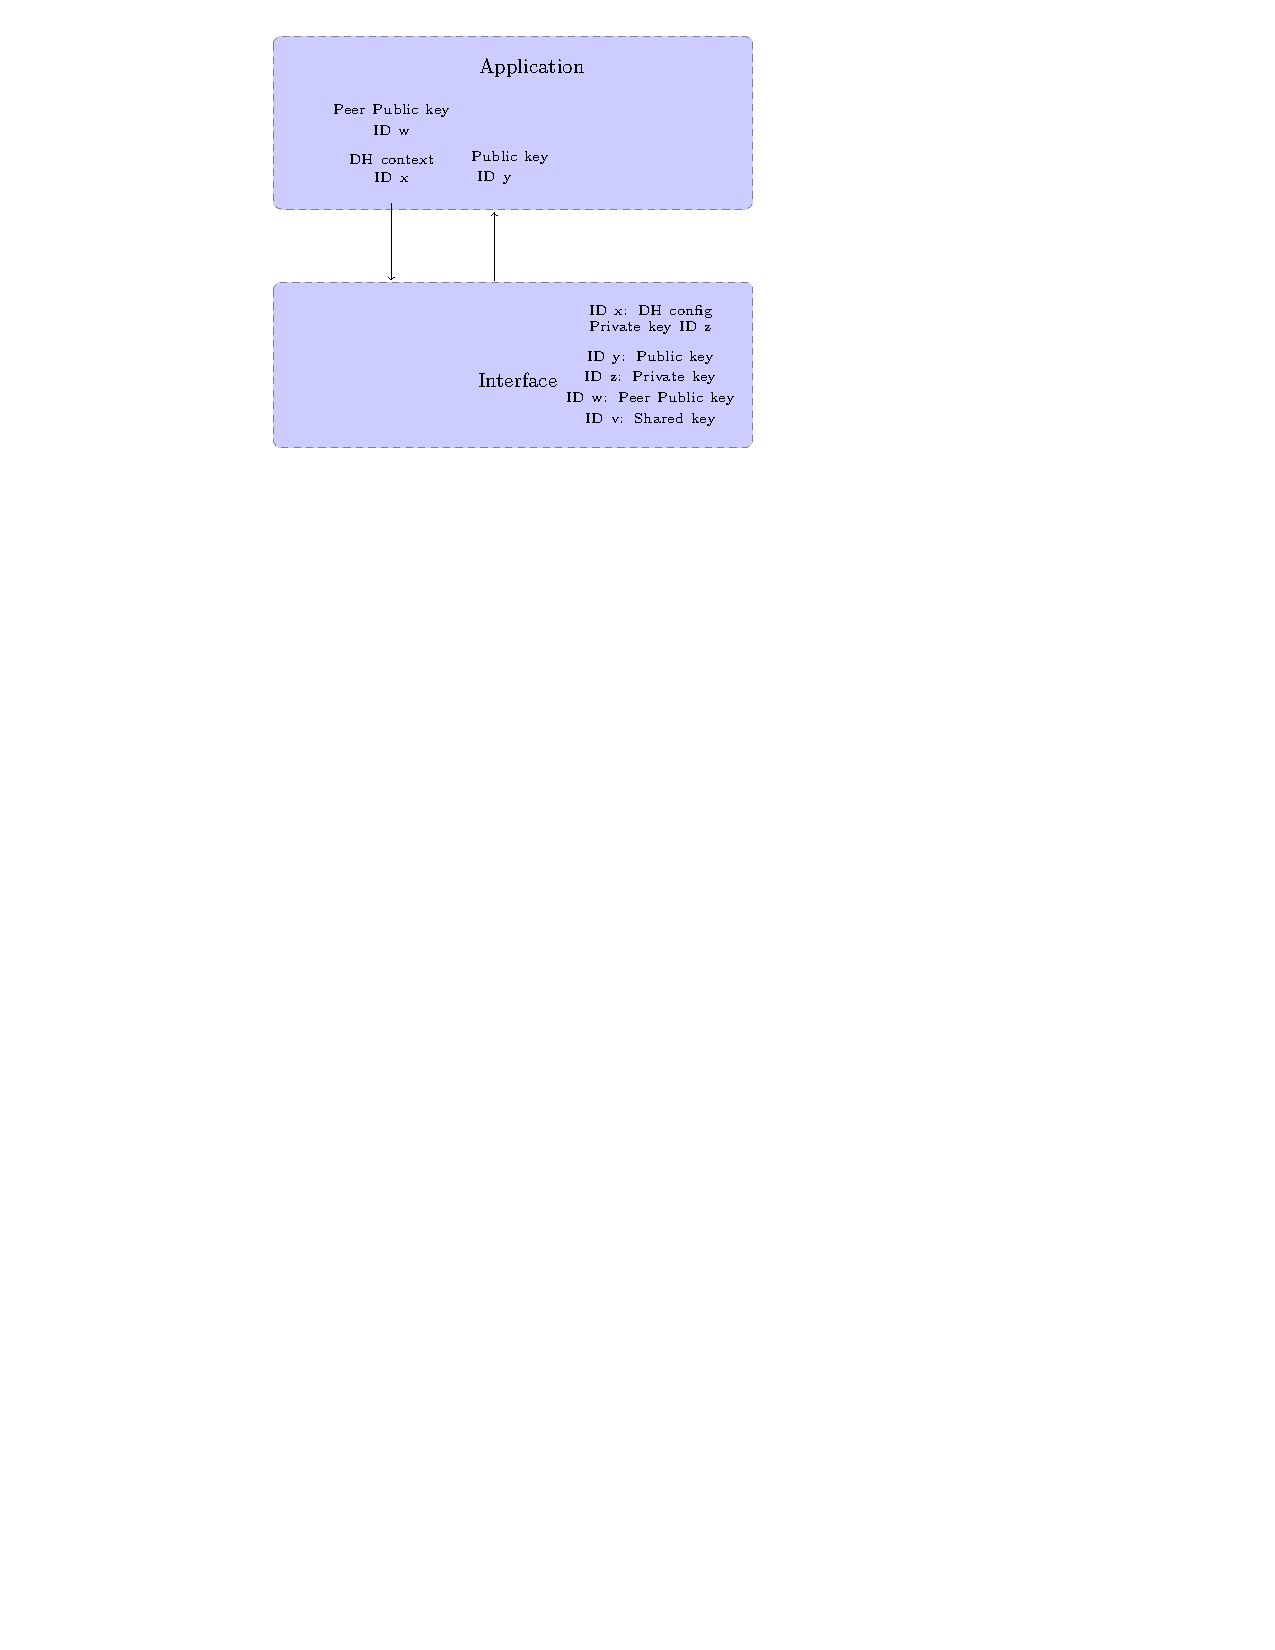
\includegraphics[trim=8.5cm 20cm 10cm 0cm]{figures/gci_dh_calc_key.pdf}
\caption{Diffie-Hellman - Calculation of the shared key\newline}
\label{fig:gci_dh_calc_key}
%}
\end{figure}


\subsection{Random number generator}
\label{gci_rng}

A random number generator is a computational or physical devices for generating
a sequence of numbers which are impossible to predict better than a random
chance.\newline
It exists two main random number generator:
\begin{enumerate}
  \item True Random Number Generators (TRNG)\newline
  Are characterized that the output cannot be reproduced. They are based on
  physical processes like semiconductor noise or clock jitter in digital
  circuits, etc..
  \item Pseudorandom Number Generators (PNRG)
  Generated sequences which are computed from an initial seed value. PRNGs
  possess good static properties, meaning their output approximates a sequence
  of true random numbers. This is shown on figure \ref{fig:gci_prng}
\end{enumerate}

For the interface, Random number generators are very important, to generate keys
or for the ciphers, for example.

For the use of a True Random Number Generator (TRNG), with hardware-based
cryptographic modules for example, only the function to get a random number is
needed.

For the use of Pseudo Random Number Generator (PRNG), with a
cryptographic software library for example, a function to generate the initial
seed value is, furthermore, needed.


\section{Clone of context}
\label{gci_cl_ctx}
As explained in \ref{gci_hash} and \ref{gci_sign_mac} when the digest (for the hash)
and the signature (for the digital signature/MAC) is calculated, no more data
can be added to the context.
This is a problem for the use of this interface in TLS projects (\embtls for
example).
Several solutions were introduced which are:
\begin{enumerate}
  \item Use two contexts at the same time.\newline
  This wasn't very efficient, because we should know at the beginning the
  number of times a digest will be calculated, which determines the amount of
  context we have to create at the beginning.
  \item Create a context when the digest is calculated.\newline
  The disadvantage of this idea was that the whole data use previously has to be
  saved. For applications, which are used in embedded systems, like \embtls, For
  systems, like embedded systems, with memory constraints, this is not possible.
  \item Clone the context. This is the solution uses for the interface.\newline
\end{enumerate}
\begin{figure}[!ht]
\centering
%\frame{
% trim: left, bottom, right, up
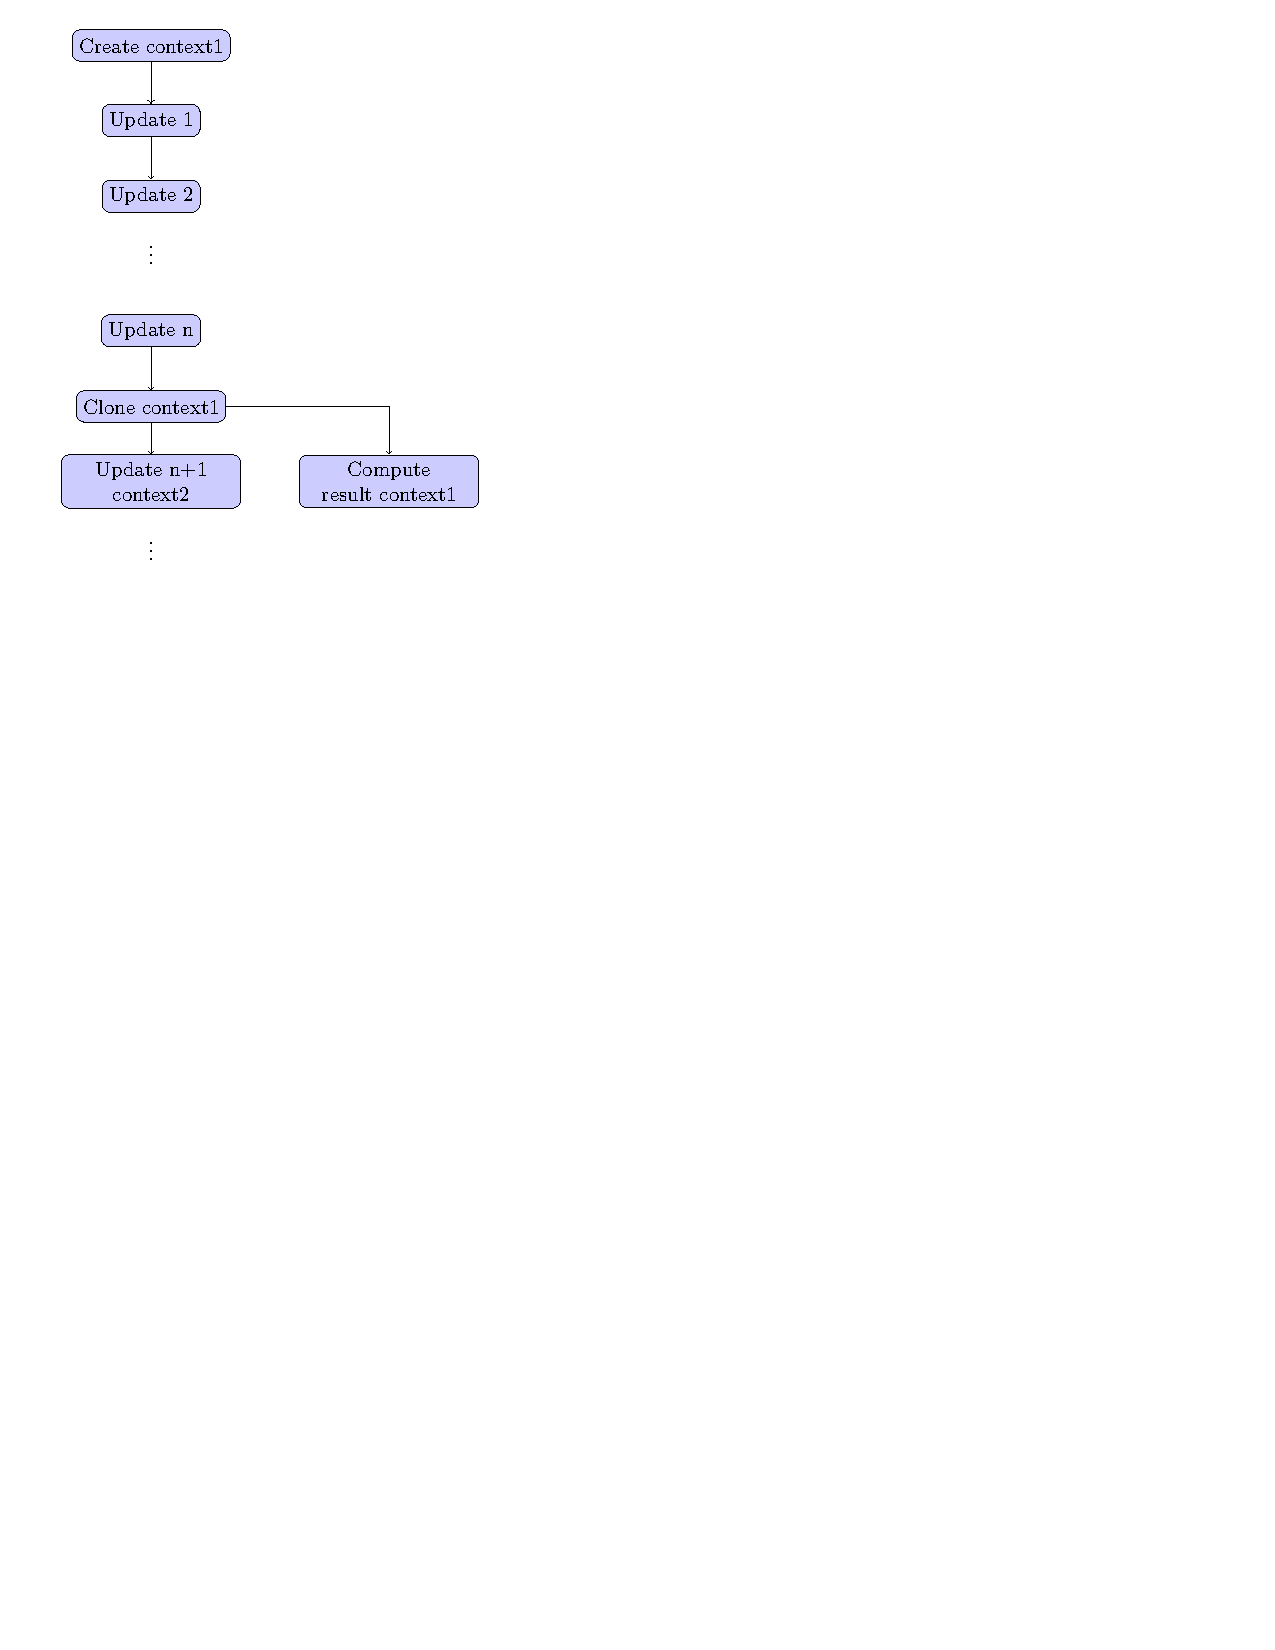
\includegraphics[trim=0cm 18.5cm 9.5cm 0cm,
height=10cm]{figures/hash_signature_clone.pdf}
\caption{Context - clone example\newline}
\label{fig:gci_clone}
%}
\end{figure}
As shown figure \ref{fig:gci_clone}, when we need to compute a result, but the
whole data added previously are needed for a future result, the solution is to
clone the context, meaning that the whole data added and the configuration is copied in another context.\newline
Then one context could be used to compute the result and the other one
to add other data when needed.\newline


\section{Key management}

\label{gci_key_mng}

In the previous version of the \embtls project interacted directly the provider
and the application.
This interaction was used for example to generate and to become directly a key
or to compute something with a key coming from the other peer.
With the interface this is not possible anymore.
That's why the key management is required for the interface.
Through the interface the keys can be saved and used by the provider to compute
something or by the application to send it to another peer.


\subsection*{Put a key}
As said in chapter \ref{gci_gen_key} Generate key pair, when a key is generated,
the ID of the key is returned to the application.
This is because the key is saved in the interface, through the function `` Put
key ``.


\begin{figure}[!ht]
\centering
%\frame{
% trim: left, bottom, right, up
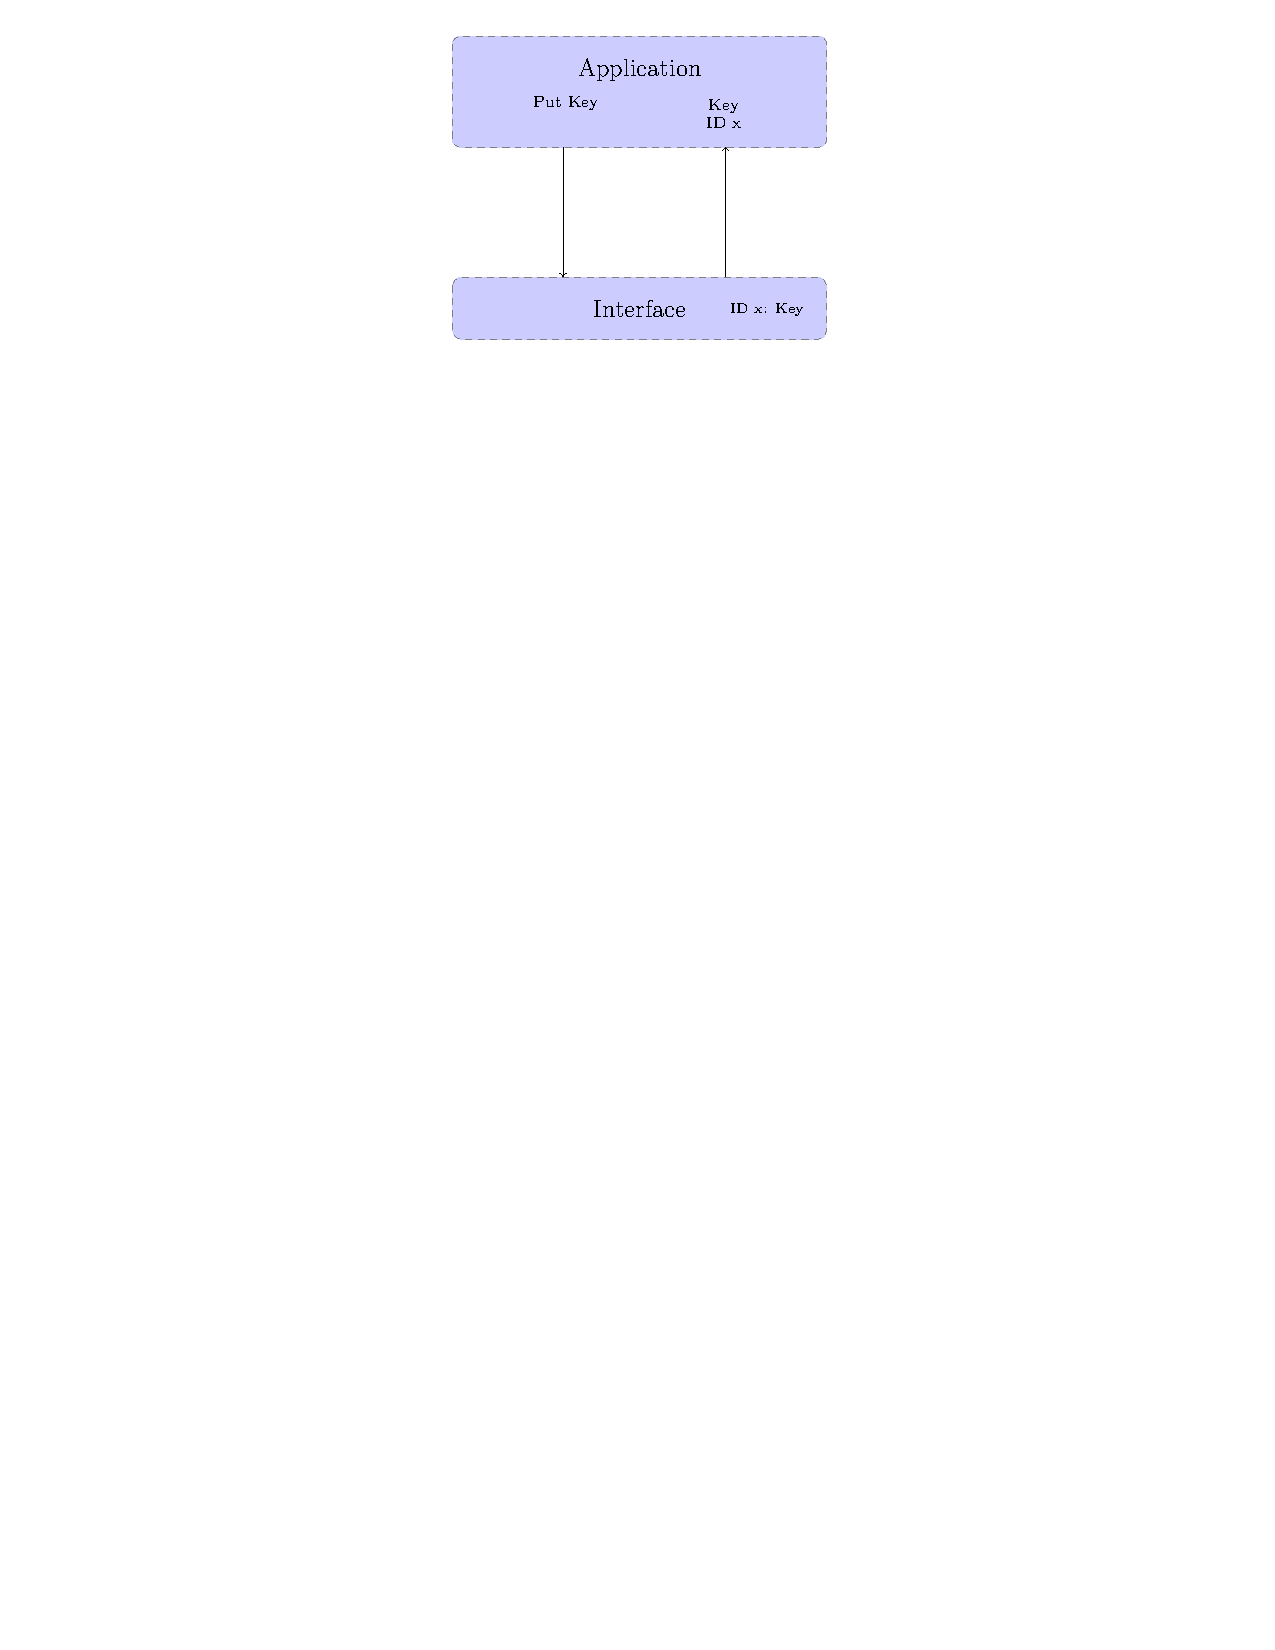
\includegraphics[trim=12cm 22cm 9.5cm 0cm]{figures/key_manag_put_key.pdf}
\caption{Key management - put a key\newline}
\label{fig:gci_key_mng_put}
%}
\end{figure}

As shown on figure \ref{fig:gci_key_mng_put}, when a key should be stored in the
interface, the key is added to the function. The interface saves it in a
specific place and return the ID of where is the key stored.


\subsection*{Get a key}
When the key should be used to be sent to another peer or to compute
something like a signature, it should be possible to get it.

\begin{figure}[!ht]
\centering
%\frame{
% trim: left, bottom, right, up
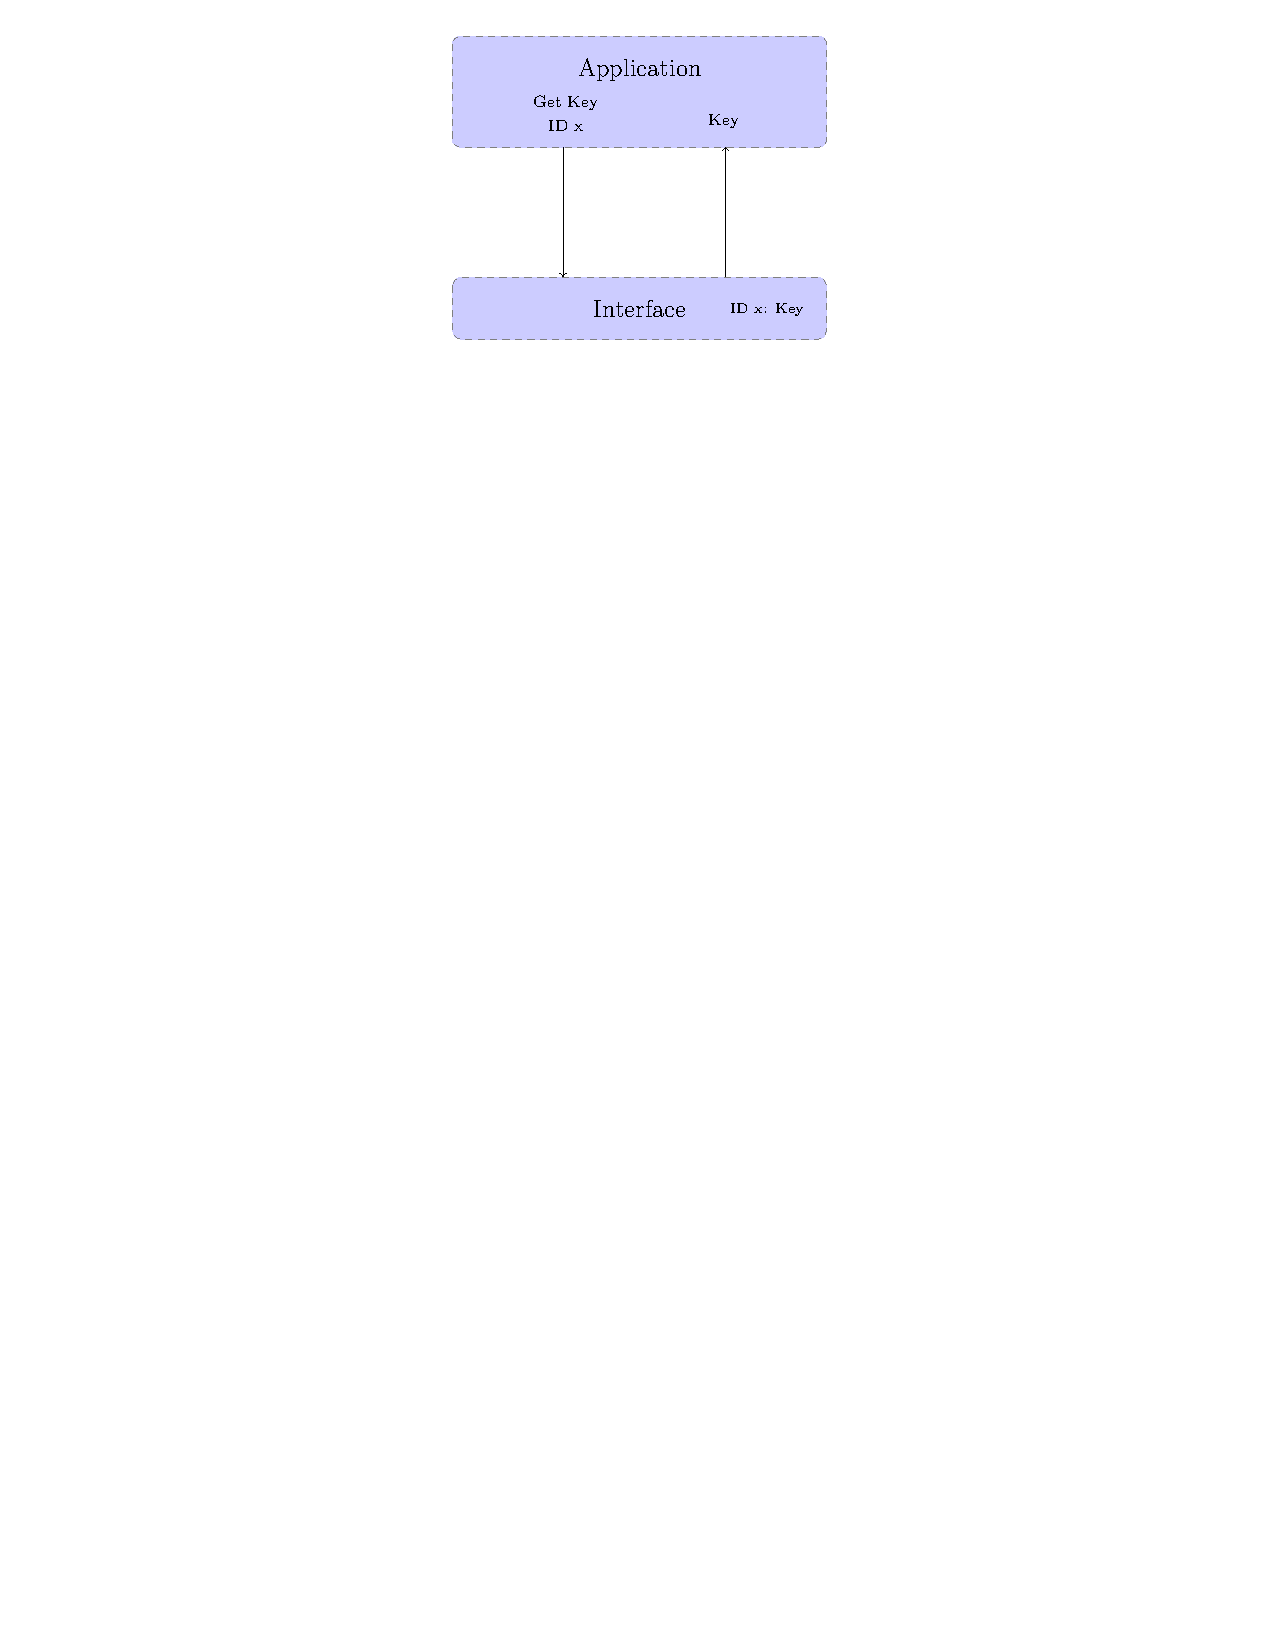
\includegraphics[trim=12cm 22cm 9.5cm 0cm]{figures/key_manag_get_key.pdf}
\caption{Key management - get a key\newline}
\label{fig:gci_key_mng_get}
%}
\end{figure}

As shown on figure \ref{fig:gci_key_mng_get}, when the key is needed by the
application, the ID should be sent the interface which will return the key
stored at this ID.

The key stays in the interface if it's still needed.

\subsection*{Delete a key}
When the key is not needed anymore, it should be possible to delete it to free
space for other keys.

\begin{figure}[!ht]
\centering
%\frame{
% trim: left, bottom, right, up
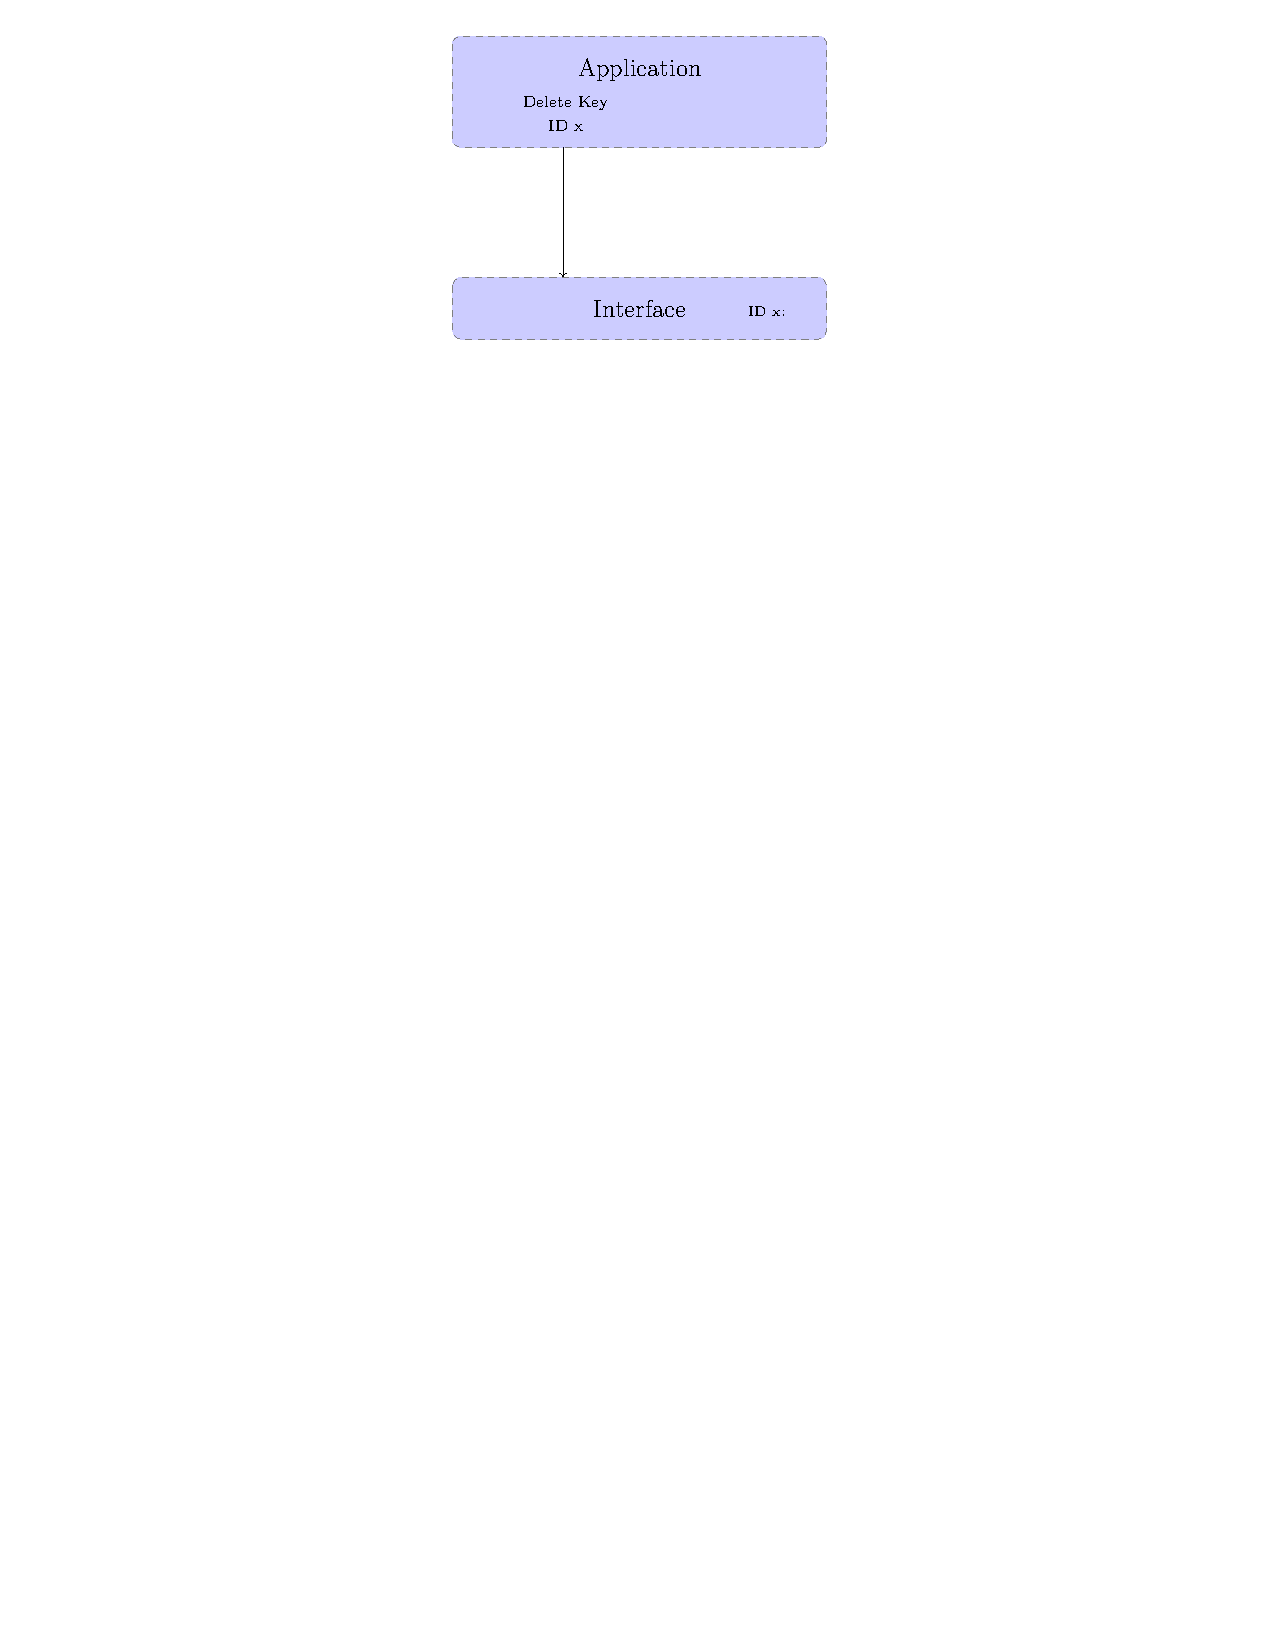
\includegraphics[trim=12cm 22cm 9.5cm 0cm]{figures/key_manag_del_key.pdf}
\caption{Key management - delete a key\newline}
\label{fig:gci_key_mng_del}
%}
\end{figure}

As shown on figure \ref{fig:gci_key_mng_del}, when the key is not needed
anymore, the ID of it is sent to the interface, which will delete it.

\chapter{Cryptography in the TLS protocol}

\section{SSL/TLS Protocol}
\label{tls_proto}

\begin{figure}[!ht]
\centering
%\frame{
% trim: left, bottom, right, up
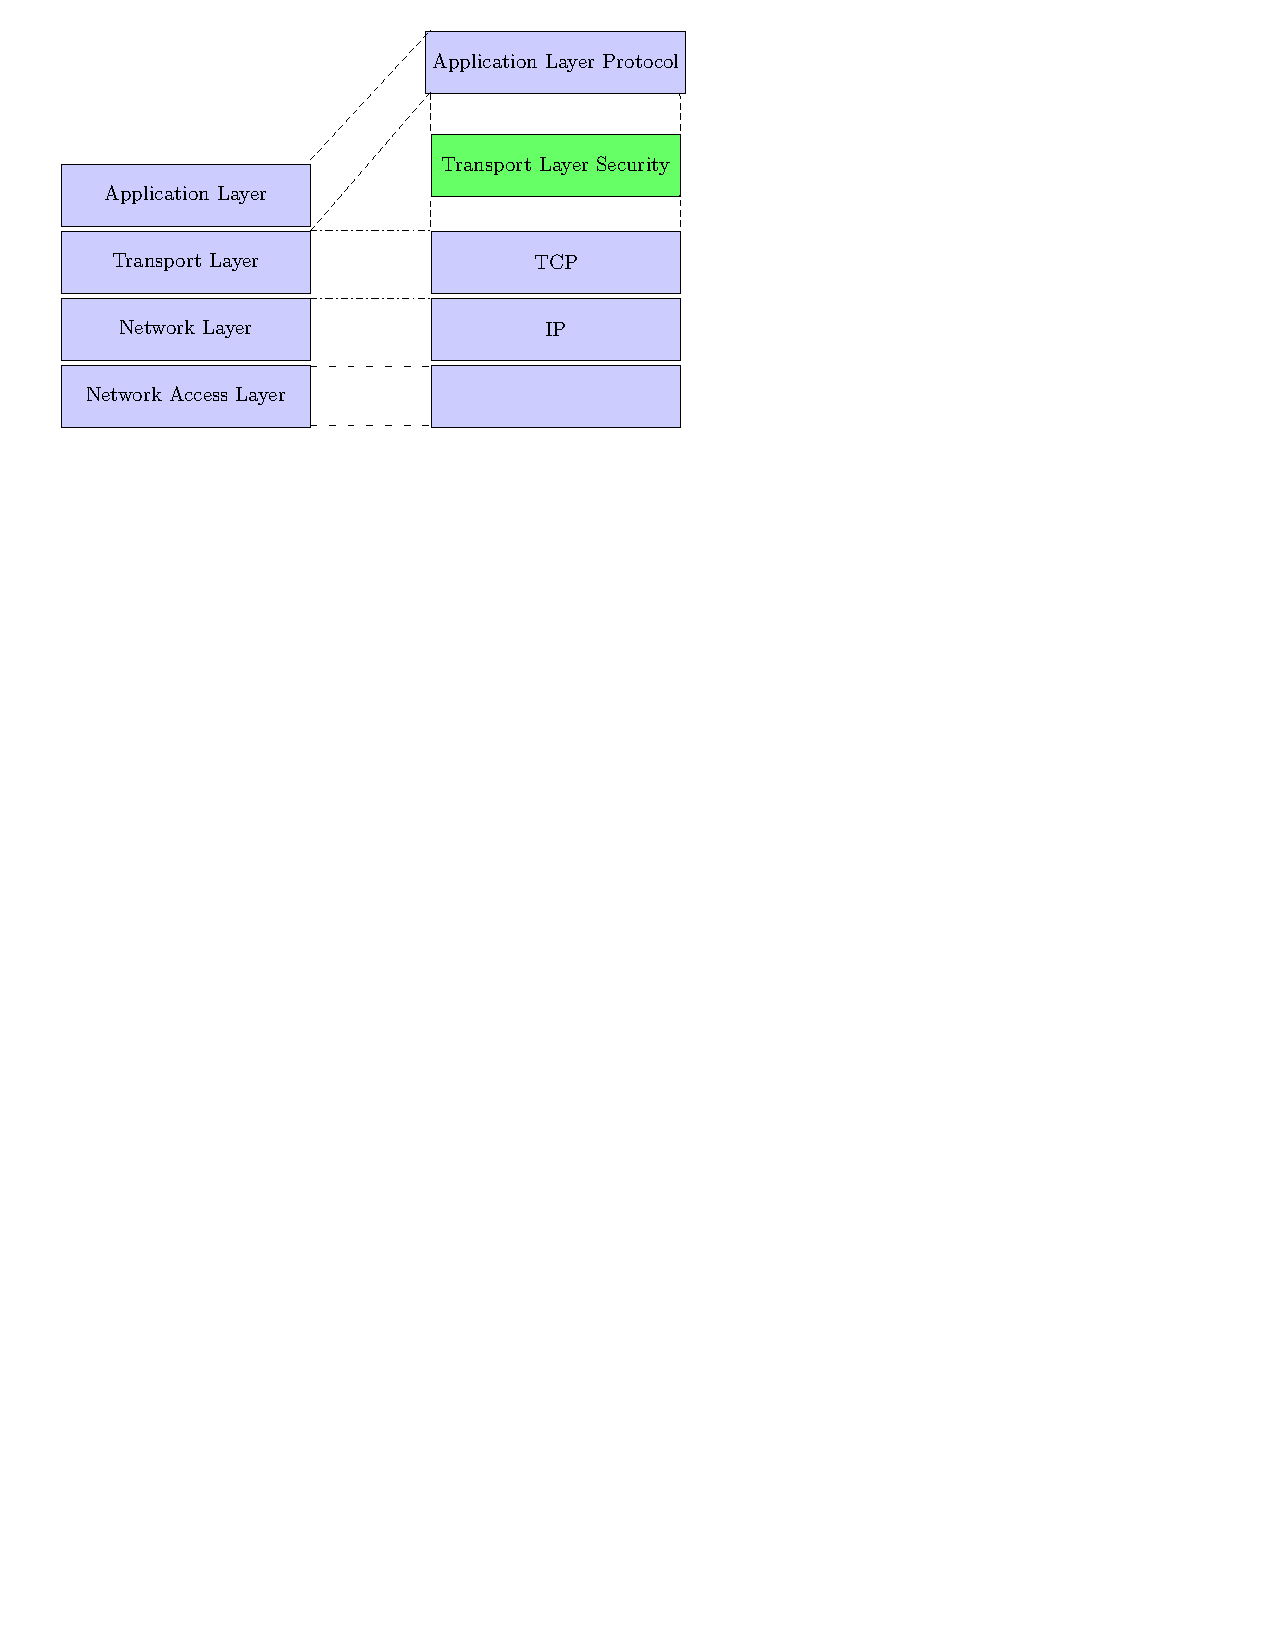
\includegraphics[trim=0cm 20.5cm 8cm 0cm]{figures/tls_osi.pdf}
\caption{TLS protocol in OSI model}
\label{fig:osi}
%}
\end{figure}

The Transport Layer Security (TLS) \cite{RFC5246}  provides communication
security, privacy and data integrity, over the Internet. Through this protocol two communicating peers
can communicate in a way which that is designed to prevent eavesdropping, tampering, or message forgery.
The TLS protocol is situated between the Application Layer and the Transport
Layer (e. g. TCP \cite{RFC0793}) in OSI model (see figure \ref{fig:osi}).

The protocol is composed of two layers
\begin{enumerate}[noitemsep]
  \item Handshake Protocol
  \item Record Protocol
\end{enumerate}

\begin{figure}[!ht]
\centering
%\frame{
% trim: left, bottom, right, up
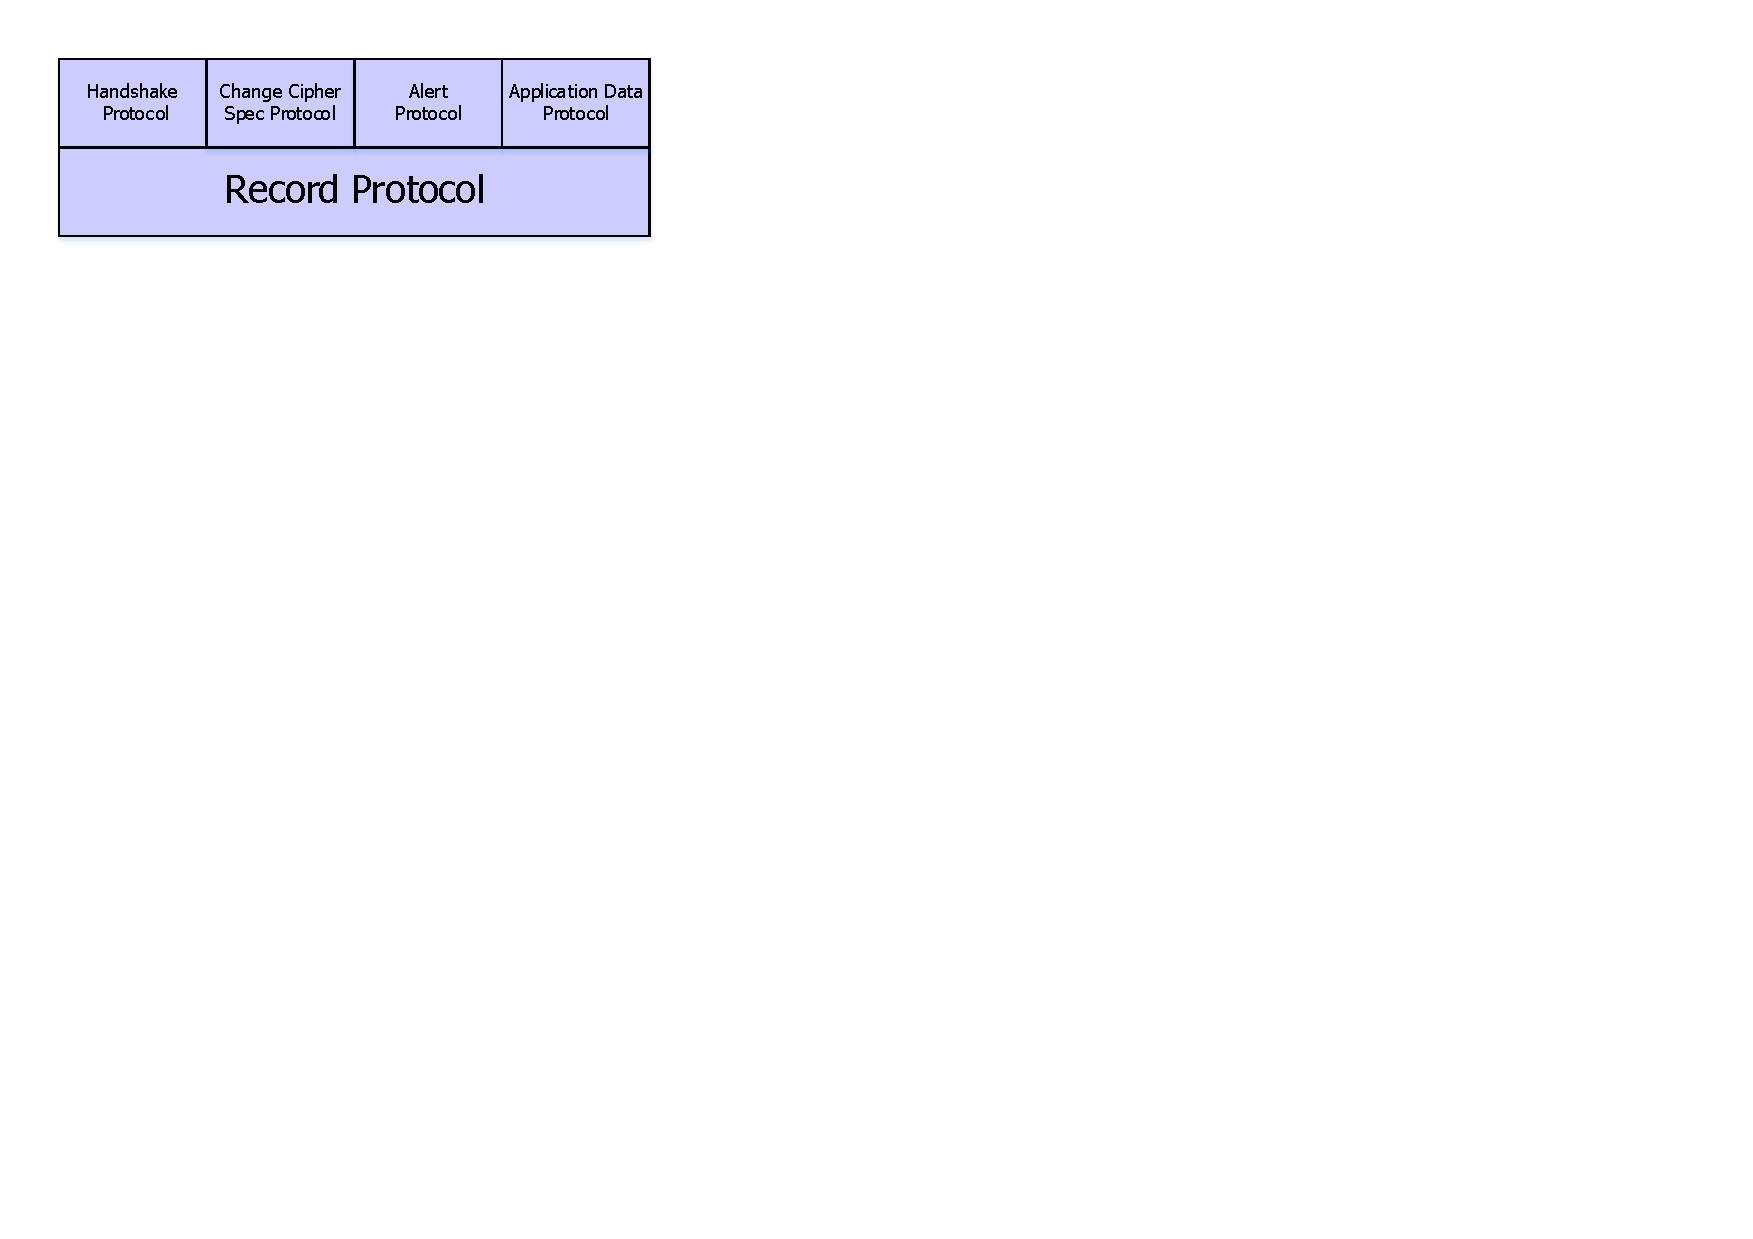
\includegraphics[trim=0cm 17cm 18cm 0cm]{figures/tls_handshake.pdf}
\caption{TLS Handshake Protocol}
\label{fig:tls_handshake}
%}
\end{figure}

\subsection{Record Protocol}

TLS Record Protocol is used for encapsulation of higher-layer protocol data,
such as TCP in case of the TCP/IP protocol \cite{RFC0793}.
It provides connection security with two basic properties:
\begin{enumerate}[noitemsep]
  \item Private connection, through symmetric cryptography algorithms (see
  section \ref{intro_sym_cipher})
  \item Reliable connection, through Message authentication Code (MAC) (see
  section \ref{intro_mac}) 
\end{enumerate}

\subsection{Handshake Protocol}

The Handshake protocol allows the two communicating peers (server and client) to
authenticate each other and to negotiate a cipher suite (see section
\ref{tls_ciph_suite}) and a compression method to transmit data.
The Handshaking Protocol is composed of four protocols:
\begin{itemize}
  \item Handshake Protocol\newline
  (See above for the definition)
  \item Change Cipher Spec Protocol\newline
  Allows to the communicating peers to signal a change of the ciphering strategy
  (see section \ref{intro_cipher})
  \item Alert Protocol\newline
  Allows the communicating peers to signal potential problems and to exchange
  corresponding alert messages
  \item Application Data Protocol\newline
  Is used for the secure transmission of application data
\end{itemize}


\subsection{Cipher suites}
\label{tls_ciph_suite}
A cipher suite \cite{RFC5246} is used to cryptographically protect data in terms
of authenticity, integrity and confidentiality.
A cipher suite allows to know which key exchange, cipher and Message
Authentication Code (MAC) will be used during the session. Figure
\ref{fig:tls_ciph_suite} shows an example of a cipher suite.\newline
 

\begin{figure}[!ht]
\centering
% trim: left, bottom, right, up
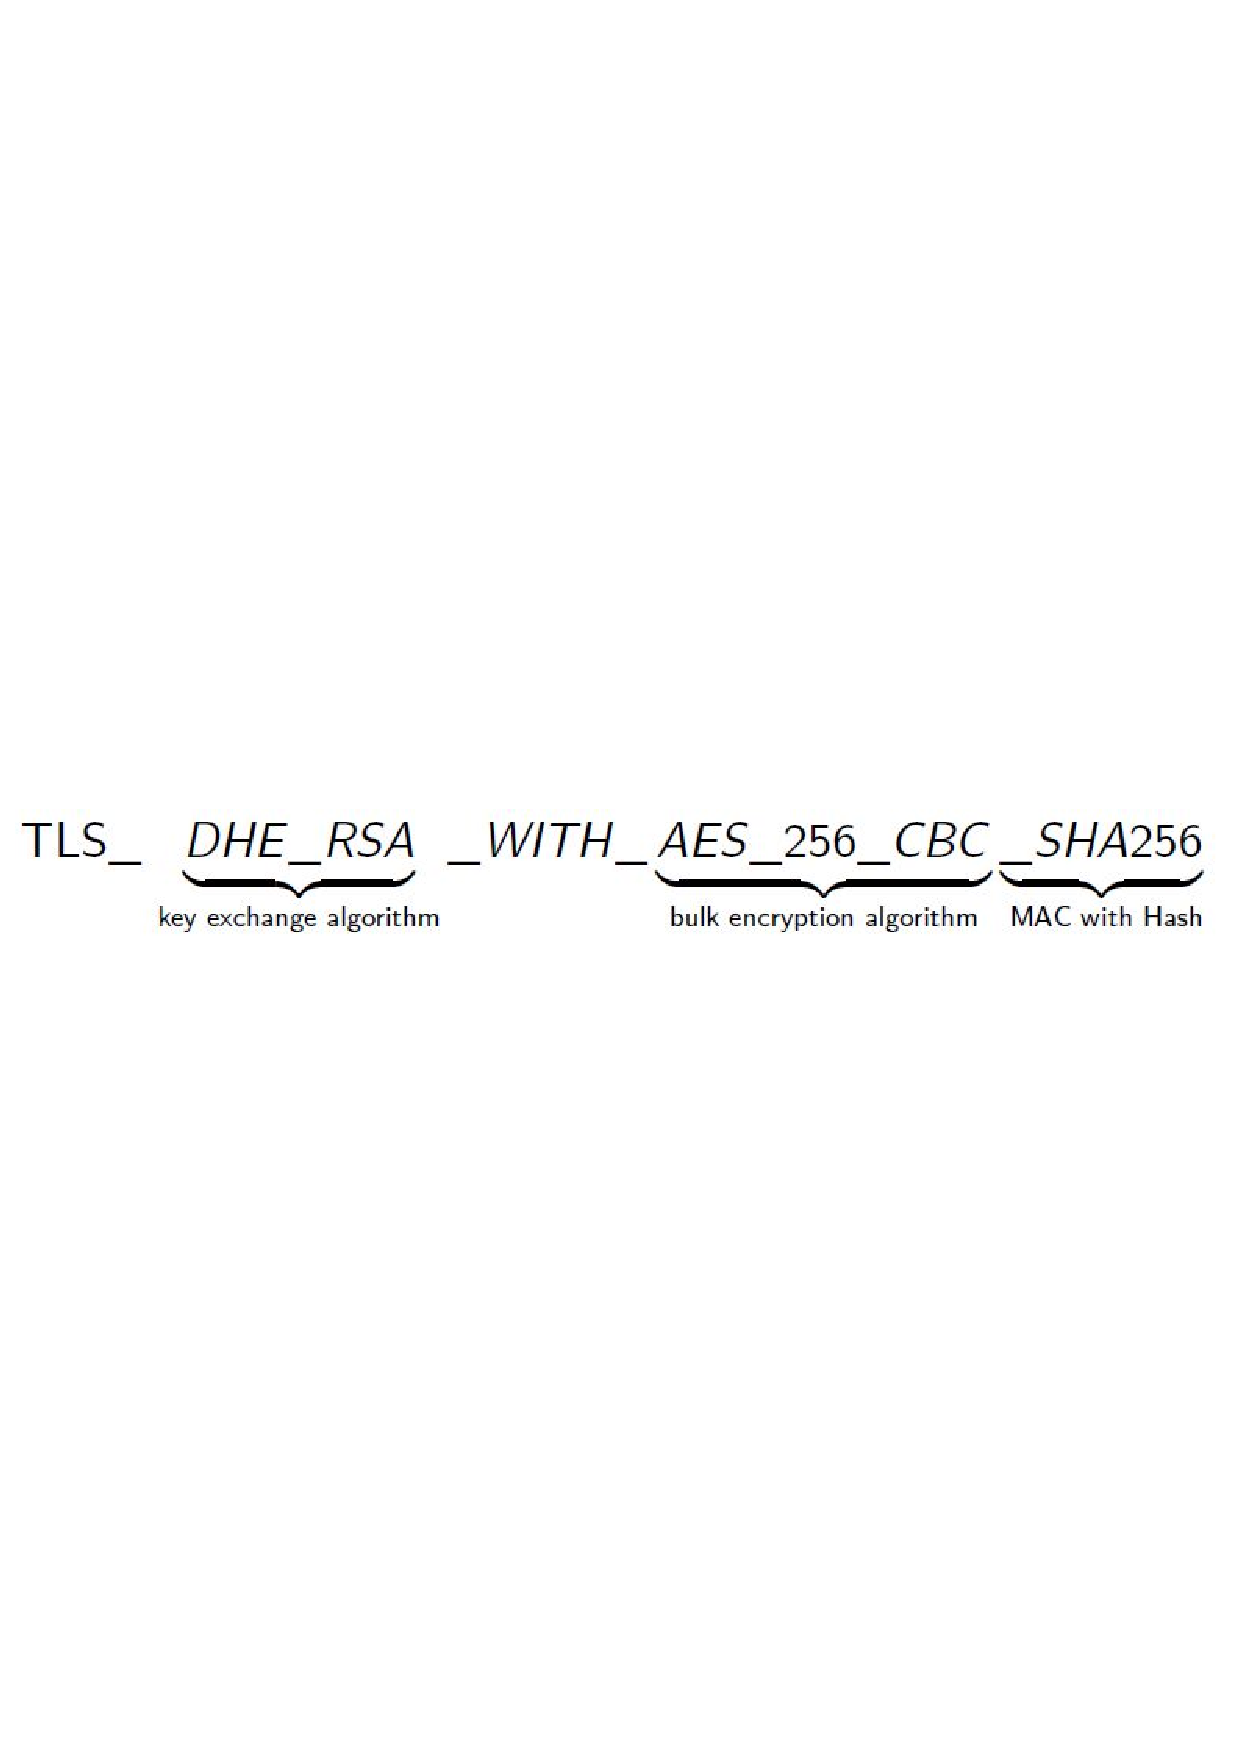
\includegraphics[trim=0cm 13.5cm 0cm 13.5cm,
height=1.75cm]{figures/tls_cipher_suite.pdf}
\caption{Example of a cipher suite}
\label{fig:tls_ciph_suite}

\end{figure}

\newpage

\section{Cryptographic parts in the Handshake Protocol}

This part describes step by step which cryptographic algorithms are used, how
they work and why these algorithms are used, for each step of the Handshake
Protocol \cite{RFC5246}.

\begin{figure}[!ht]
\centering
% trim: left, bottom, right, up
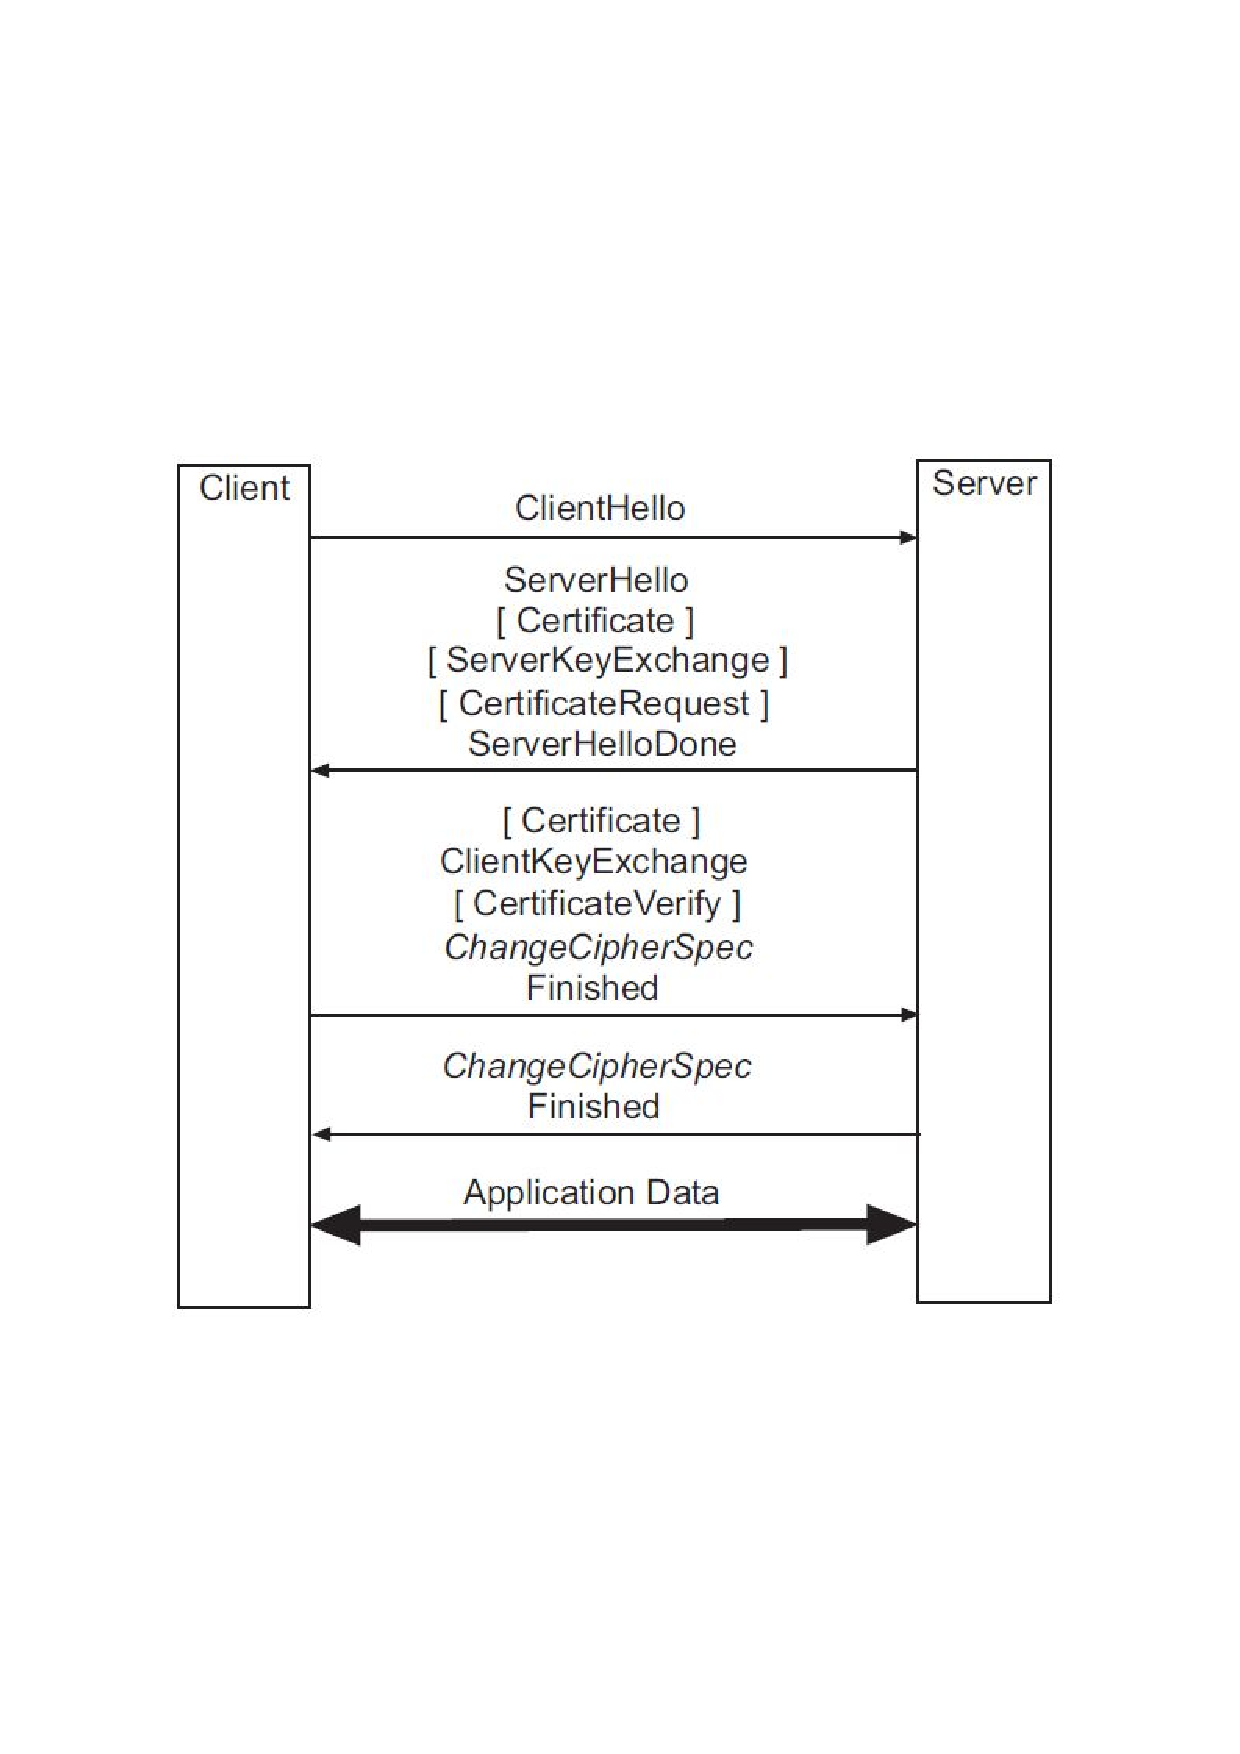
\includegraphics[trim=0cm 7cm 0cm 7cm,
height=10cm]{figures/tls_exg.pdf}
\caption{Handshake protocol (source \cite{book2})}
\label{fig:tls_exg}

\end{figure}

\subsection*{Client Hello}

A random number is generated as Client random number.

Creation of a hash function in the Client which will be used during the whole
communication.
Each received and transmitted data are added to this hash function, which allows
to be sure that the two peer has become the same data. The data of the Client
Hello are added to the hash function.

The cryptographic algorithms use in this message are:
\begin{itemize}[noitemsep]
  \item Random number (seed + random number)
  \item Hash algorithm (creation + update)
\end{itemize}


\subsection*{Server Hello}

Generation of a Server random number.
The cipher suite is chosen by the Server, which chooses with the list of cipher
suites sent by the Client in the Client Hello.

Creation of a hash function in the Server which will be used during the whole
communication.
Each received and transmitted data are added to this hash function, which allows
to be sure that the two peer has become the same data. 
The data from the Client Hello and of Server Hello are added to the hash
function.

The cryptographic algorithms use in this message are:
\begin{itemize}[noitemsep]
  \item Random number (seed + generation)
  \item Hash algorithm (creation + update)
\end{itemize}

\subsection*{Certificate}
The certificate message is sent from the Server. It contains certificates which
each one contains public key certificates which contain public keys,
digital signatures and other information.
A public key is extracted and used to verify a digital signature which
authenticate the server.
The Client can also use this public key to verify the digital signature from
the certificate and authenticates the Server.
This message is added to the Client and Server hash function.

The Client sents its certificates when a Certificate Request has been sent from
Server.

The cryptographic algorithm uses in this message is:
\begin{itemize}[noitemsep]
  \item Digital signature algorithm (verification)
  \item Hash algorithm (update)
\end{itemize}

\subsection*{Server Key Exchange}
The Server Key Exchange is sent when Diffie-Hellman or Elliptic Curve
Diffie-Hellman  is used as key exchange.
In this Server Key Exchange the domain parameters are sent, which are used to
generate the public key of the client and of the server.

The public key of the server and the private key of the public key are used to
generate the secret key.

The data of the Server Key Exchange are added to the hash function of the Client
and the Server.

The cryptographic algorithms use in this message are:
\begin{itemize}[noitemsep]
  \item Diffie-Hellman/Elliptic Curve Diffie Hellman algorithm (Generation of
  key pair + calculation of the secret key)
  \item Hash algorithm (update)
\end{itemize}

\subsection*{Certificate Request}
The Certificate Request message is used when the Server wants the certificates
of the Client to authenticate it.
The certificate message is added to the hash function of the Client and the
Server.

Ony the hash algorithm (update) is used as cryptographic algorithm for this
message.

\subsection*{Server Hello Done}
The Server Hello Done is only added to the hash function of the two peer.
Therefore is only the hash algorithm (update) used for this message.

\subsection*{Client Key Exchange}
If the RSA is used as key exchange, the premaster key is computed with the Client and Server random
number sent in the Client Hello and Server Hello with the HMAC function uses for
PRF \cite{RFC5246}.
This premaster secret is encrypted with the public key of the Server, which is
extacted from the certificate coming from the Server Hello.
Only the Server which has the private key can decrypt this premaster key.

When the Server receives the Client Key Exchange, he computes the premaster key
too. He can compare its premaster key with this one decrypted from the Client
Key Exchange.

If the Diffie-Hellman or Elliptic Curve Diffie Hellman (ECDH) is used as key
exchange, the public key generates by the Client, with the domain parameters
send in the Server Key Exchange message, is sent to the Server.
Then the Server can compute the secret key too. 

The Client Key Exchange message is added to the hash function of the Client and
the Server

The cryptographic algorithms use in this message are:
\begin{itemize}[noitemsep]
  \item Hash-based Message Authentication Code (HMAC) algorithm (Generation)
  \item Diffie-Hellman / Elliptic Curve Diffie-Hellman algorithm (Calculation of
  the secret key) if Diffie-Hellman / Elliptic Curve Diffie-Hellman is used as
  key exchange
  \item RSA algorithm (Decryption) if RSA is used as key exchange
  \item Hash algorithm (update)
\end{itemize}

\subsection*{Certificate Verify}
The Client sent a digital signature, which has been done with the private key of
the Client, to the Server, so can the Server authenticates the Client with the
public extracts from the Client certificates.
This message is added to the Client and Server hash function.

The hash algorithms use in this message are:
\begin{itemize}[noitemsep]
  \item Digital signature algorithm (Generation and verification)
  \item Hash algorithm (update)
\end{itemize}


\subsection*{Change Cipher Spec}
This message allows to the communicating peers to signal transitions in
ciphering strategies, meaning that the key exchange will be the symmetric one
chooses in the cipher suite.
No cryptographic algorithms are used for this message.


\subsection*{Finish}
This message allows to the two peers to verify that the key exchange and
authentication have been successful. The digest of the hash function uses since
the beginning of the communication is computed. A Message Authentication Code is
computed with the symmetric.
The two results are encrypted with the symmetric key and the symmetric algorithm
chooses in the cipher suite.
The other peer can then decrypt the message with its symmetric key and compare
the results.
The message is added to the hash function of the two peers.

The cryptographic algorithms use in this message are:
\begin{itemize}[noitemsep]
  \item Symmetric cipher algorithm (encryption and decryption)
  \item Message Authentication Code (generation)
  \item Hash algorithm (computing digest, update)
\end{itemize}



\subsection*{Application Data}
In this step, data can be transmitted over an insecure network without potential
security problems.
The data is signed with a Message Authentication Code (MAC) with the symmetric
key.
The data and the MAC are encrypted and decrypted with the symmetric key and the
symmetric algorithm chooses in the cipher suites.

The cryptographic algorithms use in this message are:
\begin{itemize}[noitemsep]
  \item Message Authentication Code (generation)
  \item Symmetric cipher algorithm (encryption and decryption)
\end{itemize}

\chapter{Implementation}

In this chapter what is implemented and what was the problems in the
implementation will be explained.
The implementation has been done in two parts. The first part is the
implementation of the interface in the application, \embtls, and the second part
the implementation of a provider, \tomcrypt, in the interface.

\section{Interface for an application}

The implementation of the interface for the application is, in fact, just a
change of was it was already done.
The function of the interface which was implemented are:
\begin{itemize}[noitemsep]
  \item Hash algorithm
  \item Signature algorithm (Generation and verification)
  \item Message Authentication Code (HMAC)
  \item Cipher algorithm (symmetric, asymmetric, for encryption and decryption)
  \item Random number generator
  \item Diffie Hellman (generation of key pair and calculation of the secret
  key)
  \item Key management
  \item Context management
\end{itemize}

The key pair generator function isn't used in this application, because when the
RSA, DSA or ECDSA are used as key pair exchange, the private key and public key
are in the Certificates.

All parameters in the application which need memory allocation was replaced as
well as possible with context and key management.
For the configuration of each context for any algorithm, all parameters must be
configured, and if a parameter isn't needed, this one must be configured like
``Name\_of\_the\_parameters"\_None.
Before getting an ID of a context and of a key, this ID must be equal to ``-1'',
because some context does different steps depending on the value of the incoming
ID in the interface.


The problems occurred during the implementation of the interface for the
application was:
\begin{itemize}
  \item When sending a Server Key Exchange, the parameters to send are in a
  certain order. In the old implementation, this part was
  done with functions from the provider, but these functions are not
  handled by the new interface. The solution was to rewrite this function
  but directly in the application part and without using the functions from the
  provider. To do that, the sequence to send the parameters should be known,
  which are represented in figure \ref{fig:srv_key_exg}. With the figure \ref{fig:srv_key_exg}
  and the use of the software Wireshark to understand the meaning of what was done in the
  old implementation, it was easier to rewrite this part of the Server Key Exchange.
  This problem and solution is the same for receiving a Server Key Exchange, and
  quick the same for sending and receiving the public key in the Client Key
  Exchange.
  \item When extracting the public key of a certificate, when the
  Certificates are coming from the Server, this part has been done with
  functions from the provider in the old implementation. The functions use
  ASN.1 DER encoding rules \cite{rec:der} function, which are very complex and
  this is not the goal of the project to rewrite this sort of function. That's why another
  source file, named ``gci\_tomcrypt'', has been created to use the function
  from the provider, but with the goal to not have any part of the provider written
  in the application part.
\end{itemize}


\begin{figure}[!ht]
\centering
%\frame{
% trim: left, bottom, right, up
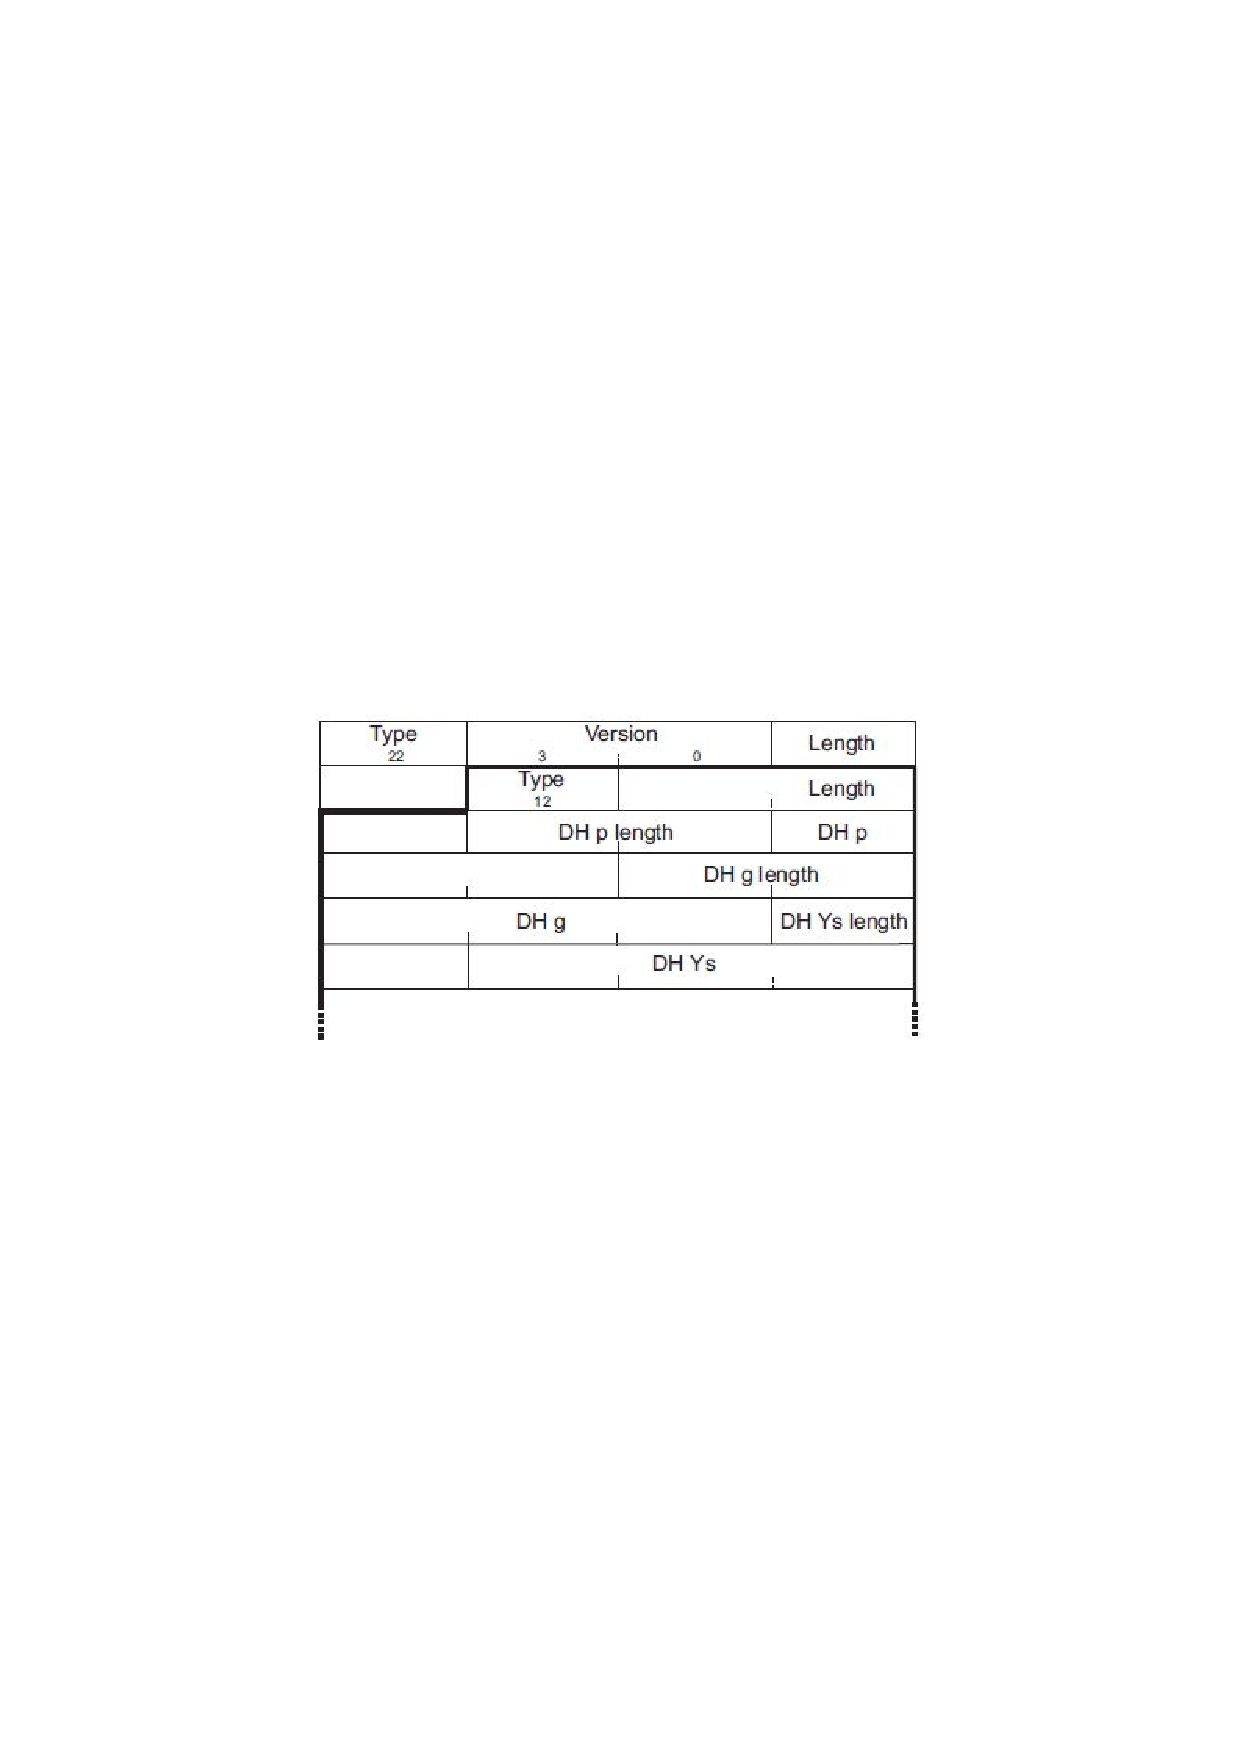
\includegraphics[trim=2cm 12cm 0cm 12cm]{figures/srv_key_exg.pdf}
\caption{Server Key Exchange - Diffie-Hellman as key exchange (source
\cite{book2})}
\label{fig:srv_key_exg}
%}
\end{figure}

\section{Provider for the interface}

The implementation of the \tomcrypt provider to the Generic Cryptographic
Interface (GCI) is important to do all the calculation needed for each algorithm
needed by the application.

For the hash algorithm context (includes the clone of the context of the hash
algorithm), the hash algorithms implemented are:
\begin{itemize}[noitemsep]
  \item MD5 algorithm, which is used by the \embtls application and works
  \item SHA1 algorithm, which is used by the \embtls application and works
  \item SHA224 algorithm, which isn't used by the \embtls application and also
  not tested
  \item SHA256 algorithm, which is used by the \embtls application and works
  \item SHA384 algorithm, which isn't used by the \embtls application and also
  not tested
  \item SHA512 algorithm, which isn't used by the \embtls application and also
  not tested
\end{itemize}

All the hash algorithms have been implemented, but not all have been tested,
because they aren't used by the \embtls application.

For the generation of the signature, the signature/Message Authentication Code
(MAC) algorithms implemented are:
\begin{itemize}[noitemsep]
  \item Hash-based Message Authentication Code (HMAC), which is used
  by the \embtls application and works
  \item RSA algorithm, which is used by the \embtls application and works
\end{itemize}

The signature/Message Authentication Code (MAC) algorithms, which aren't
implemented are:
\begin{itemize}[noitemsep]
  \item Cipher-based Message Authentication Code (CMAC)
  \item DSA
  \item ECDSA
\end{itemize}

These algorithms weren't implemented, because they aren't used by the \embtls
application.

The clone of a signature isn't implemented too, because it's not needed for the
\embtls application


For the verification of the signature, the signature/Message Authentication Code
(MAC) algorithm implemented is the hash-based Message Authentication Code
(HMAC).
The other algorithms (see above, for the generation of a signature) aren't
needed for the \embtls application.


For the generation of key pair (RSA, DSA or ECDSA) none has been implemented,
because none is needed for the \embtls application.

For the cipher (symmetric and asymmetric) algorithms, these implemented are:
\begin{itemize}[noitemsep]
  \item RC4, tested and works
  \item DES, implemented but not tested
  \item 3DES, tested and works
  \item RSA, tested and works
\end{itemize}

The block mode for the symmetric algorithms implemented are:
\begin{itemize}[noitemsep]
  \item CBC
  \item CFB
  \item ECB
  \item GCM
  \item OFB
\end{itemize}
Only the CBC block mode is used by the \embtls application, the others are
implemented, but not tested.

Generation of a Random Number (included the seed) is implemented and works

Diffie-Hellman (and Elliptic Curve of Diffie-Hellman (ECDH)) is implemented and
works.

The context management and key management are implemented and work too.

For the algorithms, which has been implemented but not tested, are implemented,
because the implementation doesn't change a lot compared to this which was
implemented and worked (Hash algorithm and Block mode for the symmetric cipher).

Problems occurred for the implementation of the \tomcrypt provider for the
Generic Cryptographic Interface:

\begin{itemize}
  \item Generation of the signature\newline
  The provider needs, of course, the private key but the public key too to
  generate the signature. In the interface, only one key at a time can be added
  to the context.
  To resolve this problem, first should a context for the
  signature be created, where the configuration of the signature and the private
  key are saved. To begin, the context ID must be initialized to ``-1". This
  context ID will, after the context is created, be greater or equal to ``0".
  Then the function to create the context should be used a second time with the context
  ID previously returned. The public key should be added at this time. The
  interface checks that the context ID is equal to ``-1'', which is not the
  case. Another context won't be created, but the public key will be added to
  the context. The context has, now, the private and public key to generate
  the signature.
  \item When the encryption of the Message Authentication Code (MAC) has to be
  done, depending on the TLS version, if it's greater or equal to TLS 1.1, an
  Initalialization Vector (IV) has to be added to the cipher context before
  encrypting.
  The problem is that, when we arrived at this step, we cannot recreate a cipher
  context with the key needed to encrypt, because this key is, at this step,
  no more available. The only solution is to use the function to create a
  context and to use the context ID returned previously, when the context was
  created with the symmetric key. The context ID is different to ``-1", also a
  new context won't be created, but the new Initialization Vector (IV)
  \cite{wiki:iv} will be added to this context.
\end{itemize}
\chapter{Results}

In this chapter, the result of the implementation will be explained.
To test the implementation, several cipher suites have been used. These cipher
suites are shown in the figure \ref{fig:res}.
As we can see, almost all cipher suites work, only the cipher suites which use
ECDSA as key exchange don't work. This is because the ECDSA implementation has
been done in another project and the merge between the two project wasn't
done, because of the time.

\begin{figure}[!ht]
\centering
%\frame{
% trim: left, bottom, right, up
\includegraphics[trim=0cm 0cm 0cm 0cm]{figures/res_cipher_suites.PNG}
\caption{Result of the implementation}
\label{fig:res}
%}
\end{figure}
\chapter{Conclusion}


\section{Achieved work}

The project is, unfortunately, not completely achieved, but globally the most
important parts are done.

The project was split into four parts.
\begin{enumerate}[noitemsep]
  \item Get the knowledge about the main cryptography part and where it could be
  used in the TLS protocol
  \item Design of the new interface
  \item Implementation of the interface into the \embtls application
  \item Implementation of the \tomcrypt provider into the Generic Cryptographic
  application
\end{enumerate}

The achieved work in this project is the design of the new Generic
Cryptographic Interface (GCI)), and globally the implementation of the interface
in the application and the implementation of the provider in the interface.

These implementations were done in two parts. The first part when the \embtls
application works as Client. The Server was done with project OpenSSL
\cite{doc:openssl}.
Figure \ref{fig:res} shows the cipher suites when the application \embtls works as
Client.
The second part of the implementation was when the \embtls application works as
Server. The Client was done with the project cURL \cite{wiki:curl}. The cipher
suites which used Diffie-Hellman and Elliptic Curve Diffie-Hellman as key exchange don't work in
this part. The problem comes when we receive the Client Key Exchange. The secret
key, we have to compute, is not the same as this coming from the Client. That
should come from the decryption of the Client Key Exchange with the private key, which
the public key is sent in the Certificates. The problem could come when we send
the Server Key Exchange, maybe there is a shift with the sent data and the
Client receives the wrong public key\ldots

\section{Future work}

The future works which could be done with this project would be to finish the
implementation of the \embtls as Server (the Diffie-Hellman and Elliptic Curve
Diffie-Hellman protocols for the key exchange, which don't work), the
implementation of the ECDSA algorithm as key exchange, which was done in another
project, the test of other cipher suites to increase the use of this new Generic
Cryptographic Interface (GCI), the test of the interface in other projects to
use all the function provides by the interface and be sure that it doesn't miss
something and the most important would be to write the documentation of the new
Generic Cryptographic Interface, for other future projects which will need this
interface as support.

\section{What I learned}
Through this thesis I learned the Cryptography, a domain I didn't know until
this thesis, or maybe only the use of the hash for the checksum. I learned the
existing main cryptography algorithms and the use of them.

I learned about the TLS protocol too. It allows me to understand all the step
needed to get a secured communication and where is the TLS protocol used today.

I learned to use the software Wireshark, which was very useful for the
implementation part, chapter \ref{imp}.

%----------------------------------------------------------------------------------------
%	Bibliography
%----------------------------------------------------------------------------------------

%% prints every entry of the bib file -- useful in a state where is no cite
%\appendix
\nocite{*}

\addcontentsline{toc}{chapter}{Bibliography}

\bibliographystyle{plainurl}

\addpart*{Bibliography}

\bibliography{bib/bibliography}


%----------------------------------------------------------------------------------------
%	Appendix
%----------------------------------------------------------------------------------------
%% add possible appendix 
\appendix
\addpart*{Appendices}

\addcontentsline{toc}{chapter}{Appendices}

\begin{appendices}
\renewcommand\thechapter{A}
\chapter{\href{../doc_GCI/doc_GCI.pdf}{Documentation Interface}}
This documentation lists all functions use in the Generic Cryptographic
Interface (GCI) and explains step by step the working of each cryptographic
services definied in the interface.\newline
\end{appendices}

%----------------------------------------------------------------------------------------
%	\end{document}
%----------------------------------------------------------------------------------------
\end{document}  
